%\RequirePackage{tikz}

%#!使用uplatex 編譯
\documentclass[uplatex,a4paper,10pt]{ujarticle}

% 図の読みこみのために
\usepackage[dvipdfmx]{graphicx}

\DeclareGraphicsExtensions{.eps,.jpg,.png,.pdf}

\usepackage{tikz}

\usepackage{settings}% 字體配置
\pagestyle{plain}
\linespread{1.0} %使用割注時請勿修改文本行距,此處爲全局行距

\usepackage{multicol}

\makeatletter
\renewcommand{\LARGE}{\@setfontsize\LARGE{16pt}{26}} 
\renewcommand{\small}{\@setfontsize\small{8pt}{10}}%
\makeatother
\renewcommand{\arraystretch}{1.0} % default is 1.0
\setlength\tabcolsep{3pt} %% 这个就是重点!!

\begin{document}

%\upstsl

%\symkm

\mcfamily

\title{\mcfamily\bfseries{up\LaTeX}{小川弘和}{SZ.CLS}{説明}}
\author{子 康}
\maketitle
\begin{center}
{\fontsize{10pt}{12}\selectfont\ttfamily
ver.1.1a
}
\end{center}
\vskip20mm

\section{緣起}
\par 本模板曾經被我用於《石頭記》垂直排版之用。現如今,將代碼托管到 GitHub ,
以供愛好者們克隆使用。
\par 本模板使用{up\LaTeX}編譯。

\section{SZ.CLS詳細説明}
\par 頭文件申明。
\begin{lstlisting}[firstnumber=1]
%   File:             ShigakuZasshi type pLaTeX class
%   First released:   2004/03/12 v0.2  小川 弘和
%		website:					http://www2.kumagaku.ac.jp/teacher/herogw/
%   Modified by:      Steve Cheung 子 康
%   Modified date:    2019/01/25 -- today 2019/05/12
%
\NeedsTeXFormat{pLaTeX2e}
\ProvidesClass{sz}[2019/05/12 v1.1b ShigakuZasshi type pLaTeX class]
\end{lstlisting}

\subsection{定義的 JIS A 系列和 B 系列紙張}
\begin{lstlisting}[firstnumber=11]
\newcounter{@paper}
\DeclareOption{a4paper}{\setcounter{@paper}{1}%
  \setlength\paperheight {297mm}%
  \setlength\paperwidth  {210mm}}
\DeclareOption{a5paper}{\setcounter{@paper}{2}%
  \setlength\paperheight {210mm}
  \setlength\paperwidth  {148mm}}
\DeclareOption{b4paper}{\setcounter{@paper}{3}%
  \setlength\paperheight {364mm}
  \setlength\paperwidth  {257mm}}
\DeclareOption{b5paper}{\setcounter{@paper}{4}%
  \setlength\paperheight {257mm}
  \setlength\paperwidth  {182mm}}
\DeclareOption{A4}{\setcounter{@paper}{1}%
  \setlength\paperheight {297mm}%
  \setlength\paperwidth  {210mm}}
\DeclareOption{A5}{\setcounter{@paper}{2}%
  \setlength\paperheight {210mm}
  \setlength\paperwidth  {148mm}}
\DeclareOption{B4}{\setcounter{@paper}{3}%
  \setlength\paperheight {364mm}
  \setlength\paperwidth  {257mm}}
\DeclareOption{B5}{\setcounter{@paper}{4}%
  \setlength\paperheight {257mm}
  \setlength\paperwidth  {182mm}}
\end{lstlisting}

\subsubsection{定義的卷子本紙張}
\par\noindent{\mc\textbf{注意:}}
\begin{itemize}
\item 定義的卷子長度不能超過 5200 mm。
%\item 卷子的長度和寬度只能有一個長邊,另一個必然是短邊。
\item 卷子的文本長度不能超過 4200 mm。
\item 定義的卷子寬度不應超過工程製圖標準紙張的高度。
\item	在main.tex中使用卷子選項\verb+[test]+。
\item 卷子的頁眉頁碼樣式要使用\verb+\pagestyle{empty}+。
\item 卷子的剪裁命令為 {\color{red}\verb+pdfcrop --margins 36  foo.pdf bar.pdf+} 。\\
其中36 表示36 pt,即0.5 inch,約爲12.5 mm。foo.pdf為裁剪的文件。
bar.pdf為保存的文件名。
\end{itemize}

\par\noindent{\mc\textbf{工程製圖標準紙張的高度。}}
\begin{biao}[高度]\leftskip 2zw
\item[A0] 高度為1070 mm。
\item[A1] 高度為 840 mm。
\item[A2] 高度為 640 mm。
\item[A3]	高度為 440 mm。
\item[A4] 高度為 300 mm。
\end{biao}

\begin{lstlisting}[firstnumber=36]
\newif\if@test \@testfalse
\DeclareOption{test}{\@testtrue\setcounter{@paper}{5}%
  \setlength\paperheight {257mm}
  \setlength\paperwidth  {5200mm}}

\if@test
	\setlength{\textheight}{4200 mm}
\fi
\end{lstlisting}

\subsection{定義的佈局}

\par 定義的雙欄和單欄,單頁佈局和對稱佈局。
\begin{lstlisting}[firstnumber=45]
\DeclareOption{onecolumn}{\@twocolumnfalse}
\DeclareOption{twocolumn}{\@twocolumntrue}
\DeclareOption{oneside}{\@twosidefalse}
\DeclareOption{twoside}{\@twosidetrue}
\end{lstlisting}

\par 定義的 landscape 佈局。
\begin{lstlisting}[firstnumber=51]
\newif\if@landscape \@landscapefalse
\DeclareOption{landscape}{\@landscapetrue
  \setlength\@tempdima{\paperheight}%
  \setlength\paperheight{\paperwidth}%
  \setlength\paperwidth{\@tempdima}}
\end{lstlisting}


\par 定義的 主要標題、副標題、作者名稱縮寫。
\begin{lstlisting}[firstnumber=58]
\def\maintitle#1{\gdef\@maintitle{#1}}
\def\@maintitle{\@latex@warning@no@line{No \noexpand\maintitle given}}

\def\subtitle#1{\gdef\@subtitle{#1}}
\def\@subtitle{\relax}

\def\authorfn#1{\gdef\@authorfn{#1}}
\def\@authorfn{\@latex@warning@no@line{No \noexpand\authorfn given}}
\end{lstlisting}

\clearpage
\par 雜項定義。
\begin{lstlisting}[firstnumber=67]
\newif\if@pdfm \@pdfmfalse
\newif\if@restonecol
\newif\if@openright
\newif\if@openleft
\newif\if@mainmatter \@mainmattertrue
\hour\time \divide\hour by 60\relax
\@tempcnta\hour \multiply\@tempcnta 60\relax
\minute\time \advance\minute-\@tempcnta
\newif\if@enablejfam \@enablejfamtrue

\DeclareOption{tombow}{%
  \tombowtrue \tombowdatetrue
  \setlength{\@tombowwidth}{.1\p@}%
  \@bannertoken{%
     \jobname\space:\space\number\year/\number\month/\number\day
      (\number\hour:\number\minute)}
  \maketombowbox}
\end{lstlisting}

\par 縱書選項。
\begin{lstlisting}[firstnumber=84]
\DeclareOption{tate}{%
  \AtBeginDocument{\tate\message{ 《縦組モード》 }%
                   \adjustbaseline}%
}
\end{lstlisting}

\subsection{定義調用字號的條件語句}
\begin{lstlisting}[firstnumber=89]
\newcounter{@fonsize}
\newif\if@setfonsizesc \@setfonsizescfalse				% 定義  9 pt(fake) 為正文字號基準,設置 mag 為 913
\newif\if@setfonsizeix \@setfonsizeixfalse				% 定義  9 pt 為正文字號基準,設置 mag 為 913
\newif\if@setfonsizex \@setfonsizexfalse					% 定義 10 pt 為正文字號基準,設置 mag 為 913
\newif\if@setfonsizexi \@setfonsizexifalse				% 定義 11 pt 為正文字號基準,設置 mag 為 913
\newif\if@setfonsizexii \@setfonsizexiifalse			% 定義 12 pt 為正文字號基準,設置 mag 為 913
\newif\if@setfonsizexz \@setfonsizexzfalse				% 定義  小四 為正文字號基準,設置 mag 為 913
%
\DeclareOption{sz}{\setcounter{@fonsize}{1}%  9 pt @ fake
\@setfonsizesctrue}
\DeclareOption{szix}{\setcounter{@fonsize}{2}%  9 pt @ real
\@setfonsizeixtrue}
\DeclareOption{szx}{\setcounter{@fonsize}{2}% 10 pt 默認
\@setfonsizextrue}
\DeclareOption{szxi}{\setcounter{@fonsize}{3}%  11 pt
\@setfonsizexitrue}
\DeclareOption{szxii}{\setcounter{@fonsize}{4}% 12 pt
\@setfonsizexiitrue}
\DeclareOption{xz}{\setcounter{@fonsize}{5}% 小四
\@setfonsizexztrue}
\end{lstlisting}


\subsection{默認佈局以及執行選項}

\par [pdfm] 選項表示調用 dvipdfmx 編譯 pdf 。
\par 行 117,執行[pdfm] 選項;	JIS B5 紙張(寬 182 mm,高 257 mm);\\\hskip2zw
定稿;左開;垂直排版;雙面對稱佈局;單欄。
\par {\mc\textbf{注意}}:使用\par
{\centering{\color{red}\verb+ptex2pdf -l -u -ot "-kanji=utf8 "  -od "-p B5" mysample+}\par}\noindent
\hspace{5.5zw}命令編譯 pdf 時,將使用 ISO B5 紙張(寬 176 mm,高 250 mm)。
\begin{lstlisting}[firstnumber=110]
\DeclareOption{pdfm}{\@pdfmtrue}
\DeclareOption{openright}{\@openrighttrue\@openleftfalse}
\DeclareOption{openleft}{\@openlefttrue\@openrightfalse}
\DeclareOption{openany}{\@openrightfalse\@openleftfalse}
\DeclareOption{disablejfam}{\@enablejfamfalse}
\DeclareOption{draft}{\setlength\overfullrule{5pt}}
\DeclareOption{final}{\setlength\overfullrule{0pt}}
\ExecuteOptions{pdfm,b5paper,final,openleft,tate,twoside,onecolumn}
\ProcessOptions\relax
\end{lstlisting}

\par 定義的編碼方式為 JT2 表示垂直排版。
\par \verb+\mag 913+ 將度量衡縮放至 0.913 倍。 
版心縮小,使得邊注區產生更大的空間。
\par 124 行和125行 將頁面還原囘標準紙。
\par 126 行定義baseline為15pt。
\begin{lstlisting}[firstnumber=121]
\def\kanjiencodingdefault{JT2}%
\kanjiencoding{\kanjiencodingdefault}%
  \mag 913 % formerly 900
  \setlength\paperwidth{1.09529\paperwidth}%
  \setlength\paperheight{1.09529\paperheight}%
  \def\n@baseline{15}%
\end{lstlisting}

\subsection{定義正文字號}

\par \verb+\mag 913 + 
參數必要的時候會挽救溢出版面的漢字,如果值為 1000,當設置頭注時,行尾就會溢出
約2個漢字並且得不到任何提示。 值為 913 正好可以解決這個 bug。 
\verb+\mag 913 + 會將原本屬於 10 pt 系列的正文字型大小放縮成 9 pt 系列。 
而此 9 pt 不是標準的小五字。

\par 根據不同的正文字號基準,使用不同的設置,詳見第\ref{sec:intro}節
(第\pageref{sec:intro} 頁)。

\subsubsection{判斷字號選項}
判斷字號選項,如未指定,則默認為 10 pt
\begin{lstlisting}[firstnumber=131]
\if@setfonsizesc  \else%
\if@setfonsizeix  \else%
 \if@setfonsizex  \else%
 	\if@setfonsizexi  \else%
 		\if@setfonsizexii  \else%
 			\if@setfonsizexz \else%
 			\@setfonsizextrue % 10 pt 默認
 		\fi	\fi \fi \fi \fi \fi
\end{lstlisting}

\subsubsection{正文字號基準為9pt(fake)}
\begin{lstlisting}[firstnumber=143]
%% 定義正文字號
\renewcommand{\normalsize}{% \normalsize=10pt@18pt
    \@setfontsize\normalsize\@xpt{18}%
  \abovedisplayskip 10\p@ \@plus2\p@ \@minus5\p@
  \abovedisplayshortskip \z@ \@plus3\p@
  \belowdisplayshortskip 6\p@ \@plus3\p@ \@minus3\p@
   \belowdisplayskip \abovedisplayskip
   \let\@listi\@listI}

\normalsize
\setbox0\hbox{\char\euc"A1A1}%
\setlength\Cht{\ht0}
\setlength\Cdp{\dp0}
\setlength\Cwd{\wd0}
\setlength\Cvs{\baselineskip}
\setlength\Chs{\wd0}

% 字號設定
\newcommand{\small}{%
  \@setfontsize\small\@ixpt{11}%
  \abovedisplayskip 8.5\p@ \@plus3\p@ \@minus4\p@
  \abovedisplayshortskip \z@ \@plus2\p@
  \belowdisplayshortskip 4\p@ \@plus2\p@ \@minus2\p@
  \def\@listi{\leftmargin\leftmargini
              \topsep 4\p@ \@plus2\p@ \@minus2\p@
              \parsep 2\p@ \@plus\p@ \@minus\p@
              \itemsep \parsep}%
  \belowdisplayskip \abovedisplayskip}

\newcommand{\footnotesize}{%
  \@setfontsize\footnotesize\@viiipt{10}%
  \abovedisplayskip 6\p@ \@plus2\p@ \@minus4\p@
  \abovedisplayshortskip \z@ \@plus\p@
  \belowdisplayshortskip 3\p@ \@plus\p@ \@minus2\p@
  \def\@listi{\leftmargin\leftmargini
              \topsep 3\p@ \@plus\p@ \@minus\p@
              \parsep 2\p@ \@plus\p@ \@minus\p@
              \itemsep \parsep}%
  \belowdisplayskip \abovedisplayskip}

% 字號設定
\newcommand{\tiny}{\@setfontsize\tiny\@viipt\@ixpt}					    %\tiny= 7pt@9pt
\newcommand{\scriptsize}{\@setfontsize\scriptsize\@xipt\@xiipt} %\scriptsize=11pt@12pt
\newcommand{\large}{\@setfontsize\large\@xiipt{18}}				      %\large= 12pt@18pt
\newcommand{\Large}{\@setfontsize\Large\@xivpt{22}}				      %\Large= 14pt@22pt
%\newcommand{\LARGE}{\@setfontsize\LARGE\@xviipt{25}}
\newcommand{\LARGE}{\@setfontsize\LARGE\@xviipt{30}}  			    %\LARGE= 17pt@30pt

	%		因正文夾注排版需要特將此設定爲 2 倍行距为宜

%\newcommand{\huge}{\@setfontsize\huge\@xxpt{28}}
\newcommand{\huge}{\@setfontsize\huge\@xxpt{30}}    				    %\huge= 20pt@30pt
%\newcommand{\Huge}{\@setfontsize\Huge\@xxvpt{33}}
\newcommand{\Huge}{\@setfontsize\Huge\@xxvpt{36}}   				    %\Huge= 25pt@36pt

\fi % from \if@setfonsizeix % 設置 正文字號基準為 9 pt(fake)
\end{lstlisting}

\subsubsection{正文字號基準為 9 pt(real)}
\begin{lstlisting}[firstnumber=199]
\if@setfonsizeix % 設置 正文字號基準為 9 pt(real)
%% 定義正文字號
\renewcommand{\normalsize}{% \normalsize = 9pt@18pt
    \@setfontsize\normalsize{9.86pt}{19.715}%
  \abovedisplayskip 10\p@ \@plus2\p@ \@minus5\p@
  \abovedisplayshortskip \z@ \@plus3\p@
  \belowdisplayshortskip 6\p@ \@plus3\p@ \@minus3\p@
   \belowdisplayskip \abovedisplayskip
   \let\@listi\@listI}

\normalsize
\setbox0\hbox{\char\euc"A1A1}%
\setlength\Cht{1.09529\ht0}
\setlength\Cdp{1.09529\dp0}
\setlength\Cwd{1.09529\wd0}
\setlength\Cvs{1.09529\baselineskip}
\setlength\Chs{1.09529\wd0}

% 字號設定
\newcommand{\small}{%  \small = 8 pt @12pt
  \@setfontsize\small{8.76pt}{13.143}%
  \abovedisplayskip 8.5\p@ \@plus3\p@ \@minus4\p@
  \abovedisplayshortskip \z@ \@plus2\p@
  \belowdisplayshortskip 4\p@ \@plus2\p@ \@minus2\p@
  \def\@listi{\leftmargin\leftmargini
              \topsep 4\p@ \@plus2\p@ \@minus2\p@
              \parsep 2\p@ \@plus\p@ \@minus\p@
              \itemsep \parsep}%
  \belowdisplayskip \abovedisplayskip}

\newcommand{\footnotesize}{% \footnotesize = 7 pt@12pt
  \@setfontsize\footnotesize{7.667pt}{13.143}%
  \abovedisplayskip 6\p@ \@plus2\p@ \@minus4\p@
  \abovedisplayshortskip \z@ \@plus\p@
  \belowdisplayshortskip 3\p@ \@plus\p@ \@minus2\p@
  \def\@listi{\leftmargin\leftmargini
              \topsep 3\p@ \@plus\p@ \@minus\p@
              \parsep 2\p@ \@plus\p@ \@minus\p@
              \itemsep \parsep}%
  \belowdisplayskip \abovedisplayskip}

% 字號設定
\newcommand{\tiny}{\@setfontsize\tiny{6.572pt}{9.858}}					    %\tiny = 6 pt@9pt
\newcommand{\scriptsize}{\@setfontsize\scriptsize{10.95pt}{13.143}} %\scriptsize=10pt@12pt
\newcommand{\large}{\@setfontsize\large{12.05pt}{19.715}}				      %\large = 11pt@18pt
\newcommand{\Large}{\@setfontsize\Large{14.24pt}{24.096}}				      %\Large = 13pt@22pt
%\newcommand{\LARGE}{\@setfontsize\LARGE\@xviipt{25}}
\newcommand{\LARGE}{\@setfontsize\LARGE{16.43pt}{30.67}}  			    %\LARGE = 15pt@28pt
%\newcommand{\huge}{\@setfontsize\huge\@xxpt{28}}
\newcommand{\huge}{\@setfontsize\huge{18.62pt}{32.86}}    				    %\huge = 17pt@30pt
%\newcommand{\Huge}{\@setfontsize\Huge\@xxvpt{33}}
\newcommand{\Huge}{\@setfontsize\Huge{21.91pt}{32.86}}   				    %\Huge = 20pt@30pt

\fi % from \if@setfonsizeix % 設置 正文字號基準為 9 pt(real)

\end{lstlisting}


\subsubsection{正文字號基準為 10 pt(默認選項)}
\begin{lstlisting}[firstnumber=254]
\if@setfonsizex % 設置 正文字號基準為 10 pt
%% 定義正文字號
\renewcommand{\normalsize}{% \normalsize = 10pt@18pt
    \@setfontsize\normalsize{10.953pt}{19.715}%
  \abovedisplayskip 10\p@ \@plus2\p@ \@minus5\p@
  \abovedisplayshortskip \z@ \@plus3\p@
  \belowdisplayshortskip 6\p@ \@plus3\p@ \@minus3\p@
   \belowdisplayskip \abovedisplayskip
   \let\@listi\@listI}

\normalsize
\setbox0\hbox{\char\euc"A1A1}%
\setlength\Cht{1.09529\ht0}
\setlength\Cdp{1.09529\dp0}
\setlength\Cwd{1.09529\wd0}
\setlength\Cvs{1.09529\baselineskip}
\setlength\Chs{1.09529\wd0}

% 字號設定
\newcommand{\small}{%  \small = 9 pt @12pt
  \@setfontsize\small{9.86pt}{13.143}%
  \abovedisplayskip 8.5\p@ \@plus3\p@ \@minus4\p@
  \abovedisplayshortskip \z@ \@plus2\p@
  \belowdisplayshortskip 4\p@ \@plus2\p@ \@minus2\p@
  \def\@listi{\leftmargin\leftmargini
              \topsep 4\p@ \@plus2\p@ \@minus2\p@
              \parsep 2\p@ \@plus\p@ \@minus\p@
              \itemsep \parsep}%
  \belowdisplayskip \abovedisplayskip}

\newcommand{\footnotesize}{% \footnotesize = 8 pt@12pt
  \@setfontsize\footnotesize{8.76pt}{13.143}%
  \abovedisplayskip 6\p@ \@plus2\p@ \@minus4\p@
  \abovedisplayshortskip \z@ \@plus\p@
  \belowdisplayshortskip 3\p@ \@plus\p@ \@minus2\p@
  \def\@listi{\leftmargin\leftmargini
              \topsep 3\p@ \@plus\p@ \@minus\p@
              \parsep 2\p@ \@plus\p@ \@minus\p@
              \itemsep \parsep}%
  \belowdisplayskip \abovedisplayskip}

% 字號設定
\newcommand{\tiny}{\@setfontsize\tiny{6.572pt}{9.858}}					 			   %\tiny = 6 pt@9pt
\newcommand{\scriptsize}{\@setfontsize\scriptsize{12.049pt}{13.143}}		 %\scriptsize=11pt@12pt
\newcommand{\large}{\@setfontsize\large{13.143pt}{19.715}}				   	   %\large = 12pt@18pt
\newcommand{\Large}{\@setfontsize\Large{15.334pt}{24.096}}				   	   %\Large = 14pt@22pt
%\newcommand{\LARGE}{\@setfontsize\LARGE\@xviipt{25}}
\newcommand{\LARGE}{\@setfontsize\LARGE{18.62pt}{32.86}}  			  			 %\LARGE = 17pt@30pt
%\newcommand{\huge}{\@setfontsize\huge\@xxpt{28}}
\newcommand{\huge}{\@setfontsize\huge{21.906pt}{32.86}}    				 			 %\huge = 20pt@30pt
%\newcommand{\Huge}{\@setfontsize\Huge\@xxvpt{33}}
\newcommand{\Huge}{\@setfontsize\Huge{27.382pt}{39.43}}   						   %\Huge = 25pt@36pt

\fi % from \if@setfonsizex % 設置 正文字號基準為 10 pt (默認)
\end{lstlisting}

\clearpage
\subsubsection{正文字號基準為 11 pt}
\begin{lstlisting}[firstnumber=309]
\if@setfonsizexi % 設置 正文字號基準為 11 pt

%% 定義正文字號
\renewcommand{\normalsize}{% \normalsize = 11pt@18pt
    \@setfontsize\normalsize{12.05pt}{19.715}%
  \abovedisplayskip 10\p@ \@plus2\p@ \@minus5\p@
  \abovedisplayshortskip \z@ \@plus3\p@
  \belowdisplayshortskip 6\p@ \@plus3\p@ \@minus3\p@
   \belowdisplayskip \abovedisplayskip
   \let\@listi\@listI}

\normalsize
\setbox0\hbox{\char\euc"A1A1}%
\setlength\Cht{1.09529\ht0}
\setlength\Cdp{1.09529\dp0}
\setlength\Cwd{1.09529\wd0}
\setlength\Cvs{1.09529\baselineskip}
\setlength\Chs{1.09529\wd0}

% 字號設定
\newcommand{\small}{%  \small = 10 pt @12pt
  \@setfontsize\small{10.953pt}{13.143}%
  \abovedisplayskip 8.5\p@ \@plus3\p@ \@minus4\p@
  \abovedisplayshortskip \z@ \@plus2\p@
  \belowdisplayshortskip 4\p@ \@plus2\p@ \@minus2\p@
  \def\@listi{\leftmargin\leftmargini
              \topsep 4\p@ \@plus2\p@ \@minus2\p@
              \parsep 2\p@ \@plus\p@ \@minus\p@
              \itemsep \parsep}%
  \belowdisplayskip \abovedisplayskip}

\newcommand{\footnotesize}{% \footnotesize = 9 pt@12pt
  \@setfontsize\footnotesize{9.86pt}{13.143}%
  \abovedisplayskip 6\p@ \@plus2\p@ \@minus4\p@
  \abovedisplayshortskip \z@ \@plus\p@
  \belowdisplayshortskip 3\p@ \@plus\p@ \@minus2\p@
  \def\@listi{\leftmargin\leftmargini
              \topsep 3\p@ \@plus\p@ \@minus\p@
              \parsep 2\p@ \@plus\p@ \@minus\p@
              \itemsep \parsep}%
  \belowdisplayskip \abovedisplayskip}

% 字號設定
\newcommand{\tiny}{\@setfontsize\tiny{6.572pt}{10}}								    %\tiny = 6 pt@9.13pt
\newcommand{\scriptsize}{\@setfontsize\scriptsize{13.143pt}{13.143}} 	%\scriptsize=12pt@12pt
\newcommand{\large}{\@setfontsize\large{14.24pt}{19.715}}				      %\large = 13pt@18pt
\newcommand{\Large}{\@setfontsize\Large{16.43pt}{24.096}}				      %\Large = 15pt@22pt
%\newcommand{\LARGE}{\@setfontsize\LARGE\@xviipt{25}}
\newcommand{\LARGE}{\@setfontsize\LARGE{18.62pt}{32.86}}  			 		  %\LARGE = 17pt@30pt
\newcommand{\huge}{\@setfontsize\huge{21.906pt}{32.86}}    				    %\huge = 20pt@30pt
\newcommand{\Huge}{\@setfontsize\Huge{27.382pt}{39.43}}   				    %\Huge = 25pt@36pt

\fi % from \if@setfonsizexi % 設置 正文字號基準為 11 pt
\end{lstlisting}


\subsubsection{正文字號基準為 12 pt}
\begin{lstlisting}[firstnumber=363]
\if@setfonsizexii  % 設置 正文字號基準為 12 pt
%% 定義正文字號
\renewcommand{\normalsize}{% \normalsize = 12pt@18pt
    \@setfontsize\normalsize{13.143pt}{19.715}%
  \abovedisplayskip 10\p@ \@plus2\p@ \@minus5\p@
  \abovedisplayshortskip \z@ \@plus3\p@
  \belowdisplayshortskip 6\p@ \@plus3\p@ \@minus3\p@
   \belowdisplayskip \abovedisplayskip
   \let\@listi\@listI}

\normalsize
\setbox0\hbox{\char\euc"A1A1}%
\setlength\Cht{1.09529\ht0}
\setlength\Cdp{1.09529\dp0}
\setlength\Cwd{1.09529\wd0}
\setlength\Cvs{1.09529\baselineskip}
\setlength\Chs{1.09529\wd0}

% 字號設定
\newcommand{\small}{%  \small = 11 pt @12pt
  \@setfontsize\small{12.05pt}{13.143}%
  \abovedisplayskip 8.5\p@ \@plus3\p@ \@minus4\p@
  \abovedisplayshortskip \z@ \@plus2\p@
  \belowdisplayshortskip 4\p@ \@plus2\p@ \@minus2\p@
  \def\@listi{\leftmargin\leftmargini
              \topsep 4\p@ \@plus2\p@ \@minus2\p@
              \parsep 2\p@ \@plus\p@ \@minus\p@
              \itemsep \parsep}%
  \belowdisplayskip \abovedisplayskip}

\newcommand{\footnotesize}{% \footnotesize = 10 pt@12pt
  \@setfontsize\footnotesize{10.95pt}{13.143}%
  \abovedisplayskip 6\p@ \@plus2\p@ \@minus4\p@
  \abovedisplayshortskip \z@ \@plus\p@
  \belowdisplayshortskip 3\p@ \@plus\p@ \@minus2\p@
  \def\@listi{\leftmargin\leftmargini
              \topsep 3\p@ \@plus\p@ \@minus\p@
              \parsep 2\p@ \@plus\p@ \@minus\p@
              \itemsep \parsep}%
  \belowdisplayskip \abovedisplayskip}

% 字號設定
\newcommand{\tiny}{\@setfontsize\tiny{8.76pt}{9.13}}					 				   %\tiny = 8 pt @ 10 pt
\newcommand{\scriptsize}{\@setfontsize\scriptsize{14.24pt}{19.715}} 	   %\scriptsize=13pt@18pt
\newcommand{\large}{\@setfontsize\large{15.334pt}{19.715}}					     %\large = 14pt@18pt
\newcommand{\Large}{\@setfontsize\Large{18.62pt}{30.67}}				      	 %\Large = 17pt@28pt
%\newcommand{\LARGE}{\@setfontsize\LARGE\@xviipt{25}}
\newcommand{\LARGE}{\@setfontsize\LARGE{21.91pt}{32.86}}  					     %\LARGE = 20pt@30pt
\newcommand{\huge}{\@setfontsize\huge{26.29pt}{32.86}}    				       %\huge = 24pt@30pt
\newcommand{\Huge}{\@setfontsize\Huge{30.67pt}{39.43}}   				    		 %\Huge = 28pt@36pt

\fi % from \if@setfonsizexii  % 設置 正文字號基準為 12 pt
\end{lstlisting}


\subsubsection{正文字號基準為 小四}
\begin{lstlisting}[firstnumber=416]
\if@setfonsizexz  % 設置 正文字號基準為 小四

%% 定義正文字號
\renewcommand{\normalsize}{% \normalsize = 10.53937pt@18pt (五號)
    \@setfontsize\normalsize{11.544pt}{19.715}%
  \abovedisplayskip 10\p@ \@plus2\p@ \@minus5\p@
  \abovedisplayshortskip \z@ \@plus3\p@
  \belowdisplayshortskip 6\p@ \@plus3\p@ \@minus3\p@
   \belowdisplayskip \abovedisplayskip
   \let\@listi\@listI}

\normalsize
\setbox0\hbox{\char\euc"A1A1}%
\setlength\Cht{1.09529\ht0}
\setlength\Cdp{1.09529\dp0}
\setlength\Cwd{1.09529\wd0}
\setlength\Cvs{1.09529\baselineskip}
\setlength\Chs{1.09529\wd0}

% 字號設定
\newcommand{\small}{%  \small = 9.03374 pt @12pt (小五)
  \@setfontsize\small{9.895pt}{13.143}%
  \abovedisplayskip 8.5\p@ \@plus3\p@ \@minus4\p@
  \abovedisplayshortskip \z@ \@plus2\p@
  \belowdisplayshortskip 4\p@ \@plus2\p@ \@minus2\p@
  \def\@listi{\leftmargin\leftmargini
              \topsep 4\p@ \@plus2\p@ \@minus2\p@
              \parsep 2\p@ \@plus\p@ \@minus\p@
              \itemsep \parsep}%
  \belowdisplayskip \abovedisplayskip}

\newcommand{\footnotesize}{% \footnotesize = 8 pt@12pt
  \@setfontsize\footnotesize{9pt}{13.143}%
  \abovedisplayskip 6\p@ \@plus2\p@ \@minus4\p@
  \abovedisplayshortskip \z@ \@plus\p@
  \belowdisplayshortskip 3\p@ \@plus\p@ \@minus2\p@
  \def\@listi{\leftmargin\leftmargini
              \topsep 3\p@ \@plus\p@ \@minus\p@
              \parsep 2\p@ \@plus\p@ \@minus\p@
              \itemsep \parsep}%
  \belowdisplayskip \abovedisplayskip}

% 字號設定
\newcommand{\tiny}{\@setfontsize\tiny{8.245pt}{10.95}}					     %\tiny = 7.52812 pt@10pt (六號)
\newcommand{\scriptsize}{\@setfontsize\scriptsize{8.762pt}{13.143}}	 %\scriptsize=8pt@12pt
\newcommand{\large}{\@setfontsize\large{13.193pt}{24.644}}	  		   %\large = 12.045pt@22.5pt (小四)
\newcommand{\Large}{\@setfontsize\Large{15.392pt}{24.644}}	  		   %\Large = 14.05249pt@22.5pt (四號)
\newcommand{\LARGE}{\@setfontsize\LARGE{16.49pt}{24.644}}  				   %\LARGE = 15.05624pt@22.5pt (小三)
%\newcommand{\huge}{\@setfontsize\huge\@xxpt{28}}
\newcommand{\huge}{\@setfontsize\huge{17.59pt}{24.644}}    				   %\huge = 16.06pt@22.5pt (三號)
%\newcommand{\Huge}{\@setfontsize\Huge\@xxvpt{33}}
\newcommand{\Huge}{\@setfontsize\Huge{19.789pt}{27.38}}   				   %\Huge = 18.06749pt@25pt (小二)

\fi % from \if@setfonsizexz  % 設置 正文字號基準為 小四
\end{lstlisting}

\subsubsection{額外定義的 小四 基準}

\par 關於 五號系列字體的定義。
\begin{lstlisting}[firstnumber=473]
\newcommand{\liuhao}{\@setfontsize\liuhao{6.572pt}{10}} % 六號
\newcommand{\xiaowu}{\@setfontsize\xiaowu{9.895pt}{13.143}} % 小五
\newcommand{\wuhao}{\@setfontsize\wuhao{11.544pt}{19.715}} % 五號
\newcommand{\xiaosi}{\@setfontsize\xiaosi{13.193pt}{24.644}} % 小四
\newcommand{\sihao}{\@setfontsize\sihao{15.392pt}{24.644}} % 四號
\newcommand{\xiaosan}{\@setfontsize\xiaosan{16.49pt}{24.644}} % 小三
\newcommand{\sanhao}{\@setfontsize\sanhao{17.59pt}{24.644}} % 三號
\newcommand{\xiaoer}{\@setfontsize\xiaoer{19.789pt}{39.43}} % 小二
\newcommand{\erhao}{\@setfontsize\erhao{24.187}{39.43}}  %(二號)
\newcommand{\xiaoyi}{\@setfontsize\xiaoyi{26.386}{39.43}}  %(小一)
\newcommand{\yihao}{\@setfontsize\yihao{28.584}{39.43}}  %(一號)
\newcommand{\xiaochu}{\@setfontsize\xiaochu{39.578}{52.57}} %(小初)
\newcommand{\chuhao}{\@setfontsize\chuhao{46.175}{52.57}} %(初號)
\end{lstlisting}


\par 【全】其他自定義的字號。
\begin{lstlisting}[firstnumber=488]
\newcommand{\bthuge}{\@setfontsize\bthuge{65.72}{78.86}}
\newcommand{\btlarge}{\@setfontsize\btlarge{52.57}{65.72}}
\newcommand{\tlarge}{\@setfontsize\tlarge{39.43}{52.57}}
\newcommand{\ularge}{\@setfontsize\ularge{32.86}{52.57}}

\newcommand{\szlarge}{%  特定的兩倍行距正文基準, \szlarge = 17 pt @ 30 pt
		\@setfontsize\szlarge{18.62pt}{32.86}%
  	\abovedisplayskip 10\p@ \@plus2\p@ \@minus5\p@
  	\abovedisplayshortskip \z@ \@plus3\p@
  	\belowdisplayshortskip 6\p@ \@plus3\p@ \@minus3\p@
   	\belowdisplayskip \abovedisplayskip%
   	\let\@listi\@listI}
\end{lstlisting}


%\clearpage
\par 古典字體設置。
\begin{lstlisting}[firstnumber=502]
\DeclareOldFontCommand{\mc}{\normalfont\mcfamily}{\mathmc}
\DeclareOldFontCommand{\gt}{\normalfont\gtfamily}{\mathgt}
\DeclareOldFontCommand{\rm}{\normalfont\rmfamily}{\mathrm}
\DeclareOldFontCommand{\sf}{\normalfont\sffamily}{\mathsf}
\DeclareOldFontCommand{\tt}{\normalfont\ttfamily}{\mathtt}
\DeclareOldFontCommand{\bf}{\normalfont\bfseries}{\mathbf}
\DeclareOldFontCommand{\it}{\normalfont\itshape}{\mathit}
\DeclareOldFontCommand{\sl}{\normalfont\slshape}{\@nomath\sl}
\DeclareOldFontCommand{\sc}{\normalfont\scshape}{\@nomath\sc}
\DeclareRobustCommand*{\cal}{\@fontswitch\relax\mathcal}
\DeclareRobustCommand*{\mit}{\@fontswitch\relax\mathnormal}
\end{lstlisting}

\subsection{引入其他依賴包}
\par 可在main.tex 中使用 \verb+\usepackage{pxfonts}+,調用 URW Palladio L 作爲西文字體。
\begin{lstlisting}[firstnumber=515]
\RequirePackage{multicol} %多欄
\RequirePackage{type1cm} %type1cm字體
\RequirePackage[expert,uplatex,deluxe]{otf} %字體包
\end{lstlisting}

\subsection{初始化各種長度變量}

\begin{lstlisting}[firstnumber=519]
\setlength\voffset{0mm}
\setlength\hoffset{0mm}

\setlength\headheight{0mm}
\setlength\headsep{0mm}

\setlength\topskip{1\Cht}
\setlength\footskip{7mm}

\setlength\maxdepth{.5\topskip}

\if@twocolumn
\setlength\textwidth{.8\paperheight}
\else
\setlength\textwidth{.8\paperheight}
\fi

\@settopoint\textwidth

\setlength\textheight{.7\paperwidth}

\addtolength\textheight{\topskip}
\@settopoint\textheight

\setlength\topmargin{-5mm}
\@settopoint\topmargin

\if@twocolumn
\setlength\marginparsep{0mm}
\else
\setlength\marginparsep{0mm}
\fi

\setlength\marginparpush{10\p@}    %%%%兩個旁注相鄰間隔

\setlength\@tempdima{\paperwidth}
\addtolength\@tempdima{-\textheight}

 \setlength\oddsidemargin{.6\@tempdima}

 \addtolength\oddsidemargin{-1in}
 \setlength\evensidemargin{\paperwidth}
 \addtolength\evensidemargin{-2in}
 \addtolength\evensidemargin{-\textheight}
 \addtolength\evensidemargin{-\oddsidemargin}
 \@settopoint\oddsidemargin % 1999.1.6
 \@settopoint\evensidemargin
 \setlength\@tempdima{\paperheight}
 \addtolength\@tempdima{-\textwidth}
 \addtolength\@tempdima{-\topmargin}
 \addtolength\@tempdima{-\headheight}
 \addtolength\@tempdima{-\headsep}
 \addtolength\@tempdima{-\footskip}
 \setlength\marginparwidth{0mm}
 \@settopoint\marginparwidth

\setlength\footnotesep{6.65\p@}
\setlength{\skip\footins}{9\p@ \@plus 4\p@ \@minus 2\p@}
\setlength\floatsep    {12\p@ \@plus 2\p@ \@minus 2\p@}
\setlength\textfloatsep{20\p@ \@plus 2\p@ \@minus 4\p@}
\setlength\intextsep   {12\p@ \@plus 2\p@ \@minus 2\p@}
\setlength\dblfloatsep    {12\p@ \@plus 2\p@ \@minus 2\p@}
\setlength\dbltextfloatsep{20\p@ \@plus 2\p@ \@minus 4\p@}
\setlength\@fptop{0\p@ \@plus 1fil}
\setlength\@fpsep{8\p@ \@plus 2fil}
\setlength\@fpbot{0\p@ \@plus 1fil}
\setlength\@dblfptop{0\p@ \@plus 1fil}
\setlength\@dblfpsep{8\p@ \@plus 2fil}
\setlength\@dblfpbot{0\p@ \@plus 1fil}
\setlength\partopsep{2\p@ \@plus 1\p@ \@minus 1\p@}
\def\@listi{\leftmargin\leftmargini
  \parsep 4\p@ \@plus2\p@ \@minus\p@
  \topsep 8\p@ \@plus2\p@ \@minus4\p@
  \itemsep4\p@ \@plus2\p@ \@minus\p@}
\let\@listI\@listi
\@listi
\def\@listii{\leftmargin\leftmarginii
   \labelwidth\leftmarginii \advance\labelwidth-\labelsep
   \topsep  4\p@ \@plus2\p@ \@minus\p@
   \parsep  2\p@ \@plus\p@  \@minus\p@
   \itemsep\parsep}
\def\@listiii{\leftmargin\leftmarginiii
   \labelwidth\leftmarginiii \advance\labelwidth-\labelsep
   \topsep 2\p@  \@plus\p@\@minus\p@
   \parsep\z@
   \partopsep \p@ \@plus\z@ \@minus\p@
   \itemsep\topsep}
\def\@listiv {\leftmargin\leftmarginiv
              \labelwidth\leftmarginiv
              \advance\labelwidth-\labelsep}
\def\@listv  {\leftmargin\leftmarginv
              \labelwidth\leftmarginv
              \advance\labelwidth-\labelsep}
\def\@listvi {\leftmargin\leftmarginvi
              \labelwidth\leftmarginvi
              \advance\labelwidth-\labelsep}
\end{lstlisting}

\subsection{重定義的cleardoublepage命令}

\begin{lstlisting}[firstnumber=616]
\def\pltx@cleartorightpage{\clearpage\if@twoside
  \ifodd\c@page
    \iftdir
      \hbox{}\thispagestyle{empty}\newpage
      \if@twocolumn\hbox{}\newpage\fi
    \fi
  \else
    \ifydir
      \hbox{}\thispagestyle{empty}\newpage
      \if@twocolumn\hbox{}\newpage\fi
    \fi
  \fi\fi}
\def\pltx@cleartoleftpage{\clearpage\if@twoside
  \ifodd\c@page
    \ifydir
      \hbox{}\thispagestyle{empty}\newpage
      \if@twocolumn\hbox{}\newpage\fi
    \fi
  \else
    \iftdir
      \hbox{}\thispagestyle{empty}\newpage
      \if@twocolumn\hbox{}\newpage\fi
    \fi
  \fi\fi}
\def\pltx@cleartooddpage{\clearpage\if@twoside
  \ifodd\c@page\else
    \hbox{}\thispagestyle{empty}\newpage
    \if@twocolumn\hbox{}\newpage\fi
  \fi\fi}
\def\pltx@cleartoevenpage{\clearpage\if@twoside
  \ifodd\c@page
    \hbox{}\thispagestyle{empty}\newpage
    \if@twocolumn\hbox{}\newpage\fi
  \fi\fi}
\if@openleft
  \let\cleardoublepage\pltx@cleartoleftpage
\else\if@openright
  \let\cleardoublepage\pltx@cleartorightpage
\fi\fi
\end{lstlisting}

\subsection{定義的另一些長度,文本框樣式}

\begin{lstlisting}[firstnumber=657]
\RequirePackage{plext}									% 縱組顓用
\RequirePackage{plautopatch}						% 為 platex 打補丁
\RequirePackage{zhnumber}								% 將數字轉化為帶單位,如 \zhnumber{9999},得九千九百九十九
%\setlength\columnsep{3\Cwd}						% 欄間距
\setlength\columnsep{2\Cwd}							% 中文縱書:欄間距 2 個全角字
\setlength\columnseprule{0\p@}					% 雙欄 欄綫設定(無欄綫)
\setlength\lineskip{1\p@}								% 行間距 1 pt
\setlength\normallineskip{1\p@}					% 正文行間距 1 pt
\renewcommand{\baselinestretch}{}				% 置空基綫距離縮放因子
\setlength\parskip{0\p@ \@plus \p@}			% 段間距 1 pt
\setlength\parindent{1\Cwd}							% 退格 1 個全角字(此處設定不會對全局縮進產生任何影響)
\setlength\marginparsep{21.9pt}					% 中文縱書:頭注與正文之間應空格 2 個全角字(即 20 pt )
\@lowpenalty   51
\@medpenalty  151
\@highpenalty 301
\setcounter{topnumber}{2}
\setcounter{bottomnumber}{1}
\setcounter{totalnumber}{3}
\setcounter{dbltopnumber}{2}
\renewcommand{\topfraction}{.7}
\renewcommand{\bottomfraction}{.3}
\renewcommand{\textfraction}{.2}
\renewcommand{\floatpagefraction}{.5}
\renewcommand{\dbltopfraction}{.7}
\renewcommand{\dblfloatpagefraction}{.5}
\end{lstlisting}

\subsection{頁眉頁碼設置 }

\par 定義兩個計數器,其中 szpage 為前言頁碼,ppage 為章回頁碼,章回頁碼要依賴章計數器。
\begin{lstlisting}[firstnumber=683]
\newcounter{chapter}
\newcounter{ppage}[chapter]
\setcounter{ppage}{1}

\newcounter{szpage}
\setcounter{szpage}{1}
\end{lstlisting}

\par 設置 plain 樣式。
\begin{lstlisting}[firstnumber=691]
%PageStyle for dvipdfmx
\if@pdfm
%\RequirePackage[dvipdfm]{graphicx}%
\RequirePackage[dvipdfmx]{graphicx}%
\def\ps@plain{%
   \let\@mkboth\markboth
   \def\@oddfoot{%
      \llap{%
         \smash{%
            \dimen@.91\textheight \advance\dimen@\footskip
            \vbox to\dimen@{%
%               \hbox{\tate \reset@font{\scriptsize\mcfamily \@maintitle ( \@authorfn ) }}%
               \hbox{\tate \reset@font{\fontsize{12pt}{14}\selectfont\gtfamily \@maintitle ( \@authorfn ) }}%
               \vfill
%               \hbox{\tate \reset@font{\small\mc \kansuji\c@page (第%
               \hbox{\tate \reset@font{\fontsize{12pt}{14}\selectfont\gtfamily \kansuji\c@page (第 %
			   \hskip.5zw{\zhnumber{\@arabic\c@ppage}}\hskip.5zw 頁)%
%               \hbox{\tate \reset@font{\scriptsize\mc \kansuji\c@page  %  此處刪去括號内頁碼
			   \vspace{25mm}}}%
			   }}%
         \hskip5mm}%
      \hfil\stepcounter{ppage}}%
      \def\chaptermark##1{ \markright{%
   \ifnum \c@secnumdepth >\m@ne
     \if@mainmatter
       \@chapapp\thechapter\@chappos\hskip1zw
     \fi
   \fi
   ##1 } }%
   \def\@evenfoot{%
      \hfil
      \rlap{%
        \hskip5mm
        \smash{%
          \dimen@.91\textheight \advance\dimen@\footskip
          \vbox to\dimen@{%
%            \hbox{\tate \reset@font{\scriptsize\mcfamily \rightmark}}%}}% 右邊頁眉設置爲章標題
            \hbox{\tate \reset@font{\fontsize{12pt}{14}\selectfont\gtfamily \rightmark}}%}}% 右邊頁眉設置爲章標題
            \vfill
%           \hbox{\tate \reset@font{\small\mc \kansuji\c@page (第%
           \hbox{\tate \reset@font{\fontsize{12pt}{14}\selectfont\gtfamily \kansuji\c@page (第%
			   \hskip.5zw{\zhnumber{\@arabic\c@ppage}}\hskip.5zw 頁)%
%         \hbox{\tate \reset@font{\scriptsize\mc \kansuji\c@page  % 此處仍刪除括號内頁碼
			   \vspace{25mm}}}}}}\stepcounter{ppage}}%
   \let\@oddhead\@empty
   \let\@evenhead\@empty
        }
\end{lstlisting}


\par 設置 前言頁碼 樣式。定義一個不包含章回標題但包含頁碼的方案。
\begin{lstlisting}[firstnumber=738]
  \def\ps@my{%
   \let\@mkboth\markboth
   \def\@oddfoot{%
      \llap{%
         \smash{%
            \dimen@.91\textheight \advance\dimen@\footskip
            \vbox to\dimen@{%
%               \hbox{\tate \reset@font{\small\mc \@maintitle ( \@authorfn ) }}%
               \vfill
%               \hbox{\tate \reset@font{\small\mc (第 \hskip.5zw{\kansuji\c@szpage}\hskip.5zw 頁) %
               \hbox{\tate \reset@font{\fontsize{12pt}{14}\selectfont\gtfamily (第 %
               \hskip.5zw{\zhnumber{\@arabic\c@szpage}}\hskip.5zw 頁) %
			   \vspace{25mm}}}%
			   }}%
         \hskip5mm}%
      \hfil\stepcounter{szpage}}%
      \def\chaptermark##1{ \markright{%
   \ifnum \c@secnumdepth >\m@ne
     \if@mainmatter
       \@chapapp\thechapter\@chappos\hskip1zw
     \fi
   \fi
   ##1 } }%
   \def\@evenfoot{%
      \hfil
      \rlap{%
        \hskip5mm
        \smash{%
          \dimen@.91\textheight \advance\dimen@\footskip
          \vbox to\dimen@{%
%            \hbox{\tate \reset@font{\small\mc \rightmark}}%}} % 右邊頁眉設置爲章標題
            \vfill
%           \hbox{\tate \reset@font{\small\mc (第 \hskip.5zw{\kansuji\c@szpage}\hskip.5zw 頁) %
           \hbox{\tate \reset@font{\fontsize{12pt}{14}\selectfont\gtfamily (第 %
           \hskip.5zw{\zhnumber{\@arabic\c@szpage}}\hskip.5zw 頁) %
			   \vspace{25mm}}}}}}\stepcounter{szpage}}%
   \let\@oddhead\@empty
   \let\@evenhead\@empty
        }
\end{lstlisting}

\par 定義用於 dvips 的頁眉頁碼。
\begin{lstlisting}[firstnumber=778]
%PageStyle for dvips
	\else
\RequirePackage[dvips]{graphicx}%
\def\ps@plain{%
   \let\@mkboth\markboth
   \def\@oddfoot{%
      \llap{%
         \smash{%
            \dimen@.91\textheight \advance\dimen@\footskip
            \vbox to\dimen@{%
               \hbox{\tate \reset@font{\scriptsize\mc \@maintitle ( \@authorfn ) }}%
               \vfill
               \hbox{\tate \reset@font{\small\mc \kansuji\c@page (第%
			   \hskip.5zw\scalebox{0.5}[1]{\kansuji\c@ppage}\hskip.5zw 頁 )%
			   \vspace{25mm}}}%
			   }}%
         \hskip5mm}%
      \hfil\stepcounter{ppage}}%
   \def\chaptermark##1{ \markright{%
   \ifnum \c@secnumdepth >\m@ne
     \if@mainmatter
       \@chapapp\thechapter\@chappos\hskip1zw
     \fi
   \fi
   ##1 } }%
   \def\@evenfoot{%
      \hfil
      \rlap{%
         \hskip5mm
         \smash{%
            \dimen@.91\textheight \advance\dimen@\footskip
            \vbox to\dimen@{%
               \hbox{\tate \reset@font{\scriptsize\mc \rightmark}}%
               \vfill
               \hbox{\tate \reset@font{\small\mc \kansuji\c@page (第%
			   \hskip.5zw\scalebox{0.5}[1]{\kansuji\c@ppage}\hskip.5zw 頁 )%
			   \vspace{25mm}}}}}}\stepcounter{ppage}}%
   \let\@oddhead\@empty
   \let\@evenhead\@empty
        }
\fi

\let\ps@jpl@in\ps@plain
\end{lstlisting}

\subsection{定義標題頁}

\par 此標題頁一般很少用到。不如直接在 main.tex 中繪製。
\begin{lstlisting}[firstnumber=822]
\def\p@thanks#1{\footnotemark
  \protected@xdef\@thanks{\@thanks
    \protect{\noindent$\m@th^\thefootnote$~#1\protect\par}}}

   \newcommand{\maketitle}{\par
  \begingroup
    \renewcommand{\thefootnote}{\fnsymbol{footnote}}%
    \def\@makefnmark{
      \ifydir
           {\leavevmode\kern-0zw\raise0.5zw\hbox{\scriptsize \@thefnmark}}
      \else
           \hbox{\yoko$\m@th^{\@thefnmark}$}
      \fi}%
    \long\def\@makefntext##1{\parindent 1zw\noindent
       \hbox to 2zw{\hss\@makefnmark}##1}%
    \if@twocolumn
      \ifnum \col@number=\@ne \@maketitle
      \else \twocolumn[\@maketitle]%
      \fi
    \else
      \newpage
      \global\@topnum\z@
      \@maketitle \cleardoublepage
    \fi

  \thispagestyle{jpl@in}\@thanks
  \endgroup
  \setcounter{footnote}{0}%
  \global\let\thanks\relax
  \global\let\maketitle\relax
  \global\let\p@thanks\relax
  \global\let\@thanks\@empty
  \global\let\@author\@empty
  \global\let\@date\@empty
  \global\let\@title\@empty
  \global\let\title\relax
  \global\let\subtitle\relax
  \global\let\author\relax
  \global\let\date\relax
  \global\let\and\relax
  }
\end{lstlisting}


\par 標題為日本史學論文風格。
\begin{lstlisting}[firstnumber=867]
\def\@maketitle{%
 \thispagestyle{empty}%
 \fboxsep5pt
    \newpage\null
  	\hspace{-1zw}{\large\mgfamily\fbox{\CID{4070}\hskip4zw\CID{3592}} \par}
			  	% \CID{4070}\CID{3592} 論文
    \vskip 4.5zw%
    \hspace{2zw}{\LARGE \@maintitle \par}%
    \vskip .5zw%
	\ifx\@subtitle\empty%
  	\hspace{6.7zw}{\large \par}%
	\else\hspace{6.7zw}{\large ------\@subtitle------ \par}\fi%
  	\vskip 4zw%
    \rightline{{\Large \@author}\hspace{4zw}}%
    \par\vskip 2zw%
   }
\end{lstlisting}

%
\subsection{文檔結構設定}

\begin{table}[H]
\begin{center}
\caption{関於編號深度的説明}
\begin{tabular}{cccc}
\hline
序號(深度) & 命令& 説明 & 對應的book標題級數 \\ \hline
-1 & \verb+\part{部標題}+ & 部、冊標題 & 一級標題 \\
0 & \verb+\chapter{章回標題}+ & 卷、章、囘標題 & 二級標題  \\
1 & \verb+\section{節標題}+ & 節標題 & 三級標題 \\
2 & \verb+\subsection{子節標題}+ & 子節標題 & 四級標題 \\
3 & \verb+\subsubsection{子小節標題}+ & 子小節標題 & 五級標題 \\ \hline
\end{tabular}
\end{center}
\end{table}

\par 可在main.tex 中使用\verb+\setcounter{secnumdepth}{x}+
改變標題編號深度。
%
\begin{lstlisting}[firstnumber=885]
\newcommand*{\chaptermark}[1]{}
\setcounter{secnumdepth}{2}			%標題編號深度

\newcounter{part}
%\newcounter{chapter}
\newcounter{section}[chapter]
\newcounter{subsection}[section]
\newcounter{subsubsection}[subsection]
\newcounter{paragraph}[subsubsection]
\newcounter{subparagraph}[paragraph]
\end{lstlisting}



\par 定義的章節數字計數器。
\begin{lstlisting}[firstnumber=896]
\renewcommand{\thepart}{\kansuji\number\@arabic\c@part}
%\renewcommand{\thechapter}{\kansuji\number\@arabic\c@chapter}
%\renewcommand{\thesection}{\kansuji\number\@arabic\c@section}
%\renewcommand{\thesubsection}{\kansuji\number\@arabic\c@subsection}

\renewcommand{\thechapter}{\zhnumber{\@arabic\c@chapter}}
\renewcommand{\thesection}{\zhnumber{\@arabic\c@section}}
\renewcommand{\thesubsection}{\zhnumber{\@arabic\c@subsection}}

\renewcommand{\thesubsubsection}{\rensuji\@arabic\c@subsubsection}
\renewcommand{\theparagraph}{\rensuji\@arabic\c@paragraph}
\renewcommand{\thesubparagraph}{\rensuji\@arabic\c@subparagraph}
\end{lstlisting}

\subsection{定義的冊卷章節}

\subsubsection{定義的冊}

\begin{lstlisting}[firstnumber=911]
\newcommand{\part}{%
  \if@openleft \cleardoublepage \else
  \if@openright \cleardoublepage \else \clearpage \fi \fi
  \thispagestyle{empty}%
  \if@twocolumn\onecolumn\@tempswatrue\else\@tempswafalse\fi
  \null\vfil
  \secdef\@part\@spart}

\def\@part[#1]#2{%
  \ifnum \c@secnumdepth >-2\relax
    \refstepcounter{part}%
    \addcontentsline{toc}{part}{%
      \mcfamily\Large \prepartname\thepart\postpartname\hspace{1em}#1}%
  \else
    \addcontentsline{toc}{part}{#1}%
  \fi
  \markboth{}{}%
  { \Huge\bfseries
   \interlinepenalty\@M\normalfont
   \ifnum \c@secnumdepth >-2\relax
   \rule{0pt}{30pt}
    \rule{30pt}{0pt}\prepartname\thepart\postpartname
     \par\vskip20\p@
   \fi
    \rule{48pt}{0pt}\Huge\bfseries#2\par}%
   \@endpart}
\def\@spart#1{{%
  \centering
  \interlinepenalty\@M\normalfont
  \Huge\bfseries#1\par}%
  \@endpart}
\def\@endpart{\vfil\newpage
  \if@twoside
   \if@openleft
    \null\thispagestyle{empty}\newpage
   \else\if@openright
    \null\thispagestyle{empty}\newpage
   \fi\fi
  \fi
   \if@tempswa\twocolumn\fi}
\end{lstlisting}


\subsubsection{定義的卷、章}

\par 自定義章標題字體,可將\verb+\mcfamily\bfseries+或者 \verb+\bfseries+
改成自定義字體的命令。
\par 定義翻一頁的章節標題,可在 行 965 行前增加 \verb+\clearpage+ 命令。
\par 正文中使用雙欄時,應在正文中使用\verb+\cleardoublepage+ 清除雙欄並翻頁。
\par 使用\verb+\usepackage{multirow}+ 和 \verb+\usepackage{multicol}+ 宏包,設置三欄時,
應使用\verb+\cleardoublepage+清除三欄並翻頁。
\begin{lstlisting}[firstnumber=953]
\newcommand{\@chapapp}{\prechaptername}
\newcommand{\@chappos}{\postchaptername}

\newcommand{\chapter}{%
  \if@openleft \cleardoublepage \else
  \if@openright \cleardoublepage \else \clearpage \fi \fi
  \global\@topnum\z@
  \@afterindenttrue
  \secdef\@chapter\@schapter  }

%%% 定義不翻頁的 章、回
\newcommand{\szchapter}{%
  \global\@topnum\z@
  \@afterindenttrue
  \secdef\@chapter\@schapter  }

%%% 章、回内部定義
\def\@chapter[#1]#2{%
  \ifnum \c@secnumdepth >\m@ne
    \if@mainmatter
    \refstepcounter{chapter}%
    \typeout{\@chapapp\space\thechapter\space\@chappos}%
    \addcontentsline{toc}{chapter}%
      {\protect\numberline{\@chapapp\thechapter\@chappos}#1}%
    \else\addcontentsline{toc}{chapter}{#1}\fi
  \else
    \addcontentsline{toc}{chapter}{#1}%
  \fi
  \chaptermark{#1}%
  \addtocontents{lof}{\protect\addvspace{10\p@}}%
  \addtocontents{lot}{\protect\addvspace{10\p@}}%
  \@makechapterhead{#2}\@afterheading}
\def\@makechapterhead#1{\hbox{}%
  \vskip.5\Cvs
  {  \hbox{\huge\textcolor{purple}{\mcfamily\bfseries \@maintitle 巻之} }
  	 % 在此處加入書籍名稱 \CID{1512}\CID{3309}  巻之
   \vskip1\Cvs
     \par \noindent \huge\mcfamily\bfseries
   \raggedright
   \leavevmode
   \ifnum \c@secnumdepth >\m@ne
     \setlength\@tempdima{\linewidth}%
    \if@mainmatter
     \setbox\z@\hbox{\@chapapp\thechapter\@chappos\hskip1zw}
     \addtolength\@tempdima{-\wd\z@}%
     \unhbox\z@\nobreak
    \fi
     \vtop{\hsize\@tempdima#1}%
   \else
     #1\relax
   \fi}\nobreak\vskip2\Cvs%
   \setcounter{ppage}{1}}
\def\@schapter#1{%
  \@makeschapterhead{#1}\@afterheading
}
\def\@makeschapterhead#1{\hbox{}%
  \vskip1\Cvs
  {\parindent\z@
   \raggedright
   \normalfont\huge\bfseries
   \leavevmode
   \setlength\@tempdima{\linewidth}%
   \vtop{\hsize\@tempdima#1}}\vskip2\Cvs}
\end{lstlisting}


\subsubsection{定義的三級、四級和五級標題}

\par 自定義章標題字體,可將\verb+\bfseries+ 改成自定義字體的命令。
\begin{lstlisting}[firstnumber=1018]
\newcommand{\section}{\@startsection{section}{1}{\z@}%
   {1.5\Cvs \@plus.5\Cvs \@minus.2\Cvs}%
   {.5\Cvs \@plus.3\Cvs}%
   {\normalfont\Large\bfseries}}
\newcommand{\subsection}{\@startsection{subsection}{2}{\z@}%
   {1.5\Cvs \@plus.5\Cvs \@minus.2\Cvs}%
   {.5\Cvs \@plus.3\Cvs}%
   {\normalfont\large\bfseries}}
\newcommand{\subsubsection}{\@startsection{subsubsection}{3}{\z@}%
   {1.5\Cvs \@plus.5\Cvs \@minus.2\Cvs}%
   {.5\Cvs \@plus.3\Cvs}%
   {\normalfont\normalsize\bfseries}}
\newcommand{\paragraph}{\@startsection{paragraph}{4}{\z@}%
   {3.25ex \@plus 1ex \@minus .2ex}%
   {-1em}%
   {\normalfont\normalsize\bfseries}}
\newcommand{\subparagraph}{\@startsection{subparagraph}{5}{\z@}%
   {3.25ex \@plus 1ex \@minus .2ex}%
   {-1em}%
   {\normalfont\normalsize\bfseries}}
\end{lstlisting}

\subsection{定義的附錄}

\begin{lstlisting}[firstnumber=1039]
\newcommand{\appendix}{\par
  \setcounter{chapter}{0}%
  \setcounter{section}{0}%
        {\appendixname}  \space%
  \renewcommand{\thechapter}{\@Kanji\c@chapter}}
\end{lstlisting}

\subsection{看不懂的長度變量和標簽序號}

\begin{lstlisting}[firstnumber=1045]
\if@twocolumn
  \setlength\leftmargini {2em}
\else
  \setlength\leftmargini {2.5em}
\fi
\setlength\leftmarginii  {2.2em}
\setlength\leftmarginiii {1.87em}
\setlength\leftmarginiv  {1.7em}
\if@twocolumn
  \setlength\leftmarginv {.5em}
  \setlength\leftmarginvi{.5em}
\else
  \setlength\leftmarginv {1em}
  \setlength\leftmarginvi{1em}
\fi
\setlength  \labelsep  {.5em}
\setlength  \labelwidth{\leftmargini}
\addtolength\labelwidth{-\labelsep}
\@beginparpenalty -\@lowpenalty
\@endparpenalty   -\@lowpenalty
\@itempenalty     -\@lowpenalty
\renewcommand{\theenumi}{\rensuji{\@arabic\c@enumi}}
\renewcommand{\theenumii}{\rensuji{(\@alph\c@enumii)}}
\renewcommand{\theenumiii}{\rensuji{\@roman\c@enumiii}}
\renewcommand{\theenumiv}{\rensuji{\@Alph\c@enumiv}}
\newcommand{\labelenumi}{\theenumi}
\newcommand{\labelenumii}{\theenumii}
\newcommand{\labelenumiii}{\theenumiii}
\newcommand{\labelenumiv}{\theenumiv}
\renewcommand{\p@enumii}{\theenumi}
\renewcommand{\p@enumiii}{\theenumi(\theenumii)}
\renewcommand{\p@enumiv}{\p@enumiii\theenumiii}
\end{lstlisting}



\subsection{定義的各種環境}

\subsubsection{定義的數字列表環境}
\begin{lstlisting}[firstnumber=1079]
\renewenvironment{enumerate}
  {\ifnum \@enumdepth >\thr@@\@toodeep\else
   \advance\@enumdepth\@ne
   \edef\@enumctr{enum\romannumeral\the\@enumdepth}%
   \list{\csname label\@enumctr\endcsname}{%
      \iftdir
         \ifnum \@listdepth=\@ne \topsep.5\normalbaselineskip
           \else\topsep\z@\fi
         \parskip\z@ \itemsep\z@ \parsep\z@
         \labelwidth1zw \labelsep.3zw
         \ifnum \@enumdepth=\@ne \leftmargin1zw\relax
           \else\leftmargin\leftskip\fi
         \advance\leftmargin 1zw
      \fi
         \usecounter{\@enumctr}%
         \def\makelabel##1{\hss\llap{##1}}}%
   \fi}{\endlist}
\newcommand{\labelitemi}{\textbullet}
\newcommand{\labelitemii}{%
  \iftdir
     {\textcircled{~}}
  \else
     {\normalfont\bfseries\textendash}
  \fi
}
\newcommand{\labelitemiii}{\textasteriskcentered}
\newcommand{\labelitemiv}{\textperiodcentered}
\end{lstlisting}


\subsubsection{定義的無序列表描述環境一}

\par 使用時以 \verb+\begin{biao}[字字字字字字]\end{biao}+作爲框架;[字字字字字字]
,全角字的個數作爲關鍵詞的寬度,默認為五個漢字的寬度。\verb+\item[関鍵詞]+調用加粗明朝字。
\begin{lstlisting}[firstnumber=1108]
\def\biao{\@ifnextchar[{\@biao}{ \@biao[ 無指定五字 ]}}
\def\@biao[#1]{%
 \list{}{%
 \let\makelabel\biaolabel\settowidth{\labelwidth}{#1}%
 \setlength{\topsep}{0pt}\setlength{\partopsep}{0pt}%
 \setlength{\parsep}{0pt}\setlength{\labelsep}{1zw}%
 \addtolength{\labelsep}{2\kanjiskip}%
 \setlength{\leftmargin}{\labelwidth}\addtolength{\leftmargin}{1zw}%
 \addtolength{\leftmargin}{2\kanjiskip}
 \setlength{\itemsep}{0pt}\setlength{\itemindent}{0pt}}}%
\let\endbiao\endlist
\def\biaolabel#1{\bfseries#1\hfill\inhibitglue}%
\end{lstlisting}

\subsubsection{定義的無序列表描述環境二}

\begin{lstlisting}[firstnumber=1121]
\renewenvironment{itemize}
  {\ifnum \@itemdepth >\thr@@\@toodeep\else
   \advance\@itemdepth\@ne
   \edef\@itemitem{labelitem\romannumeral\the\@itemdepth}%
   \expandafter
   \list{\csname \@itemitem\endcsname}{%
      \iftdir
         \ifnum \@listdepth=\@ne \topsep.5\normalbaselineskip
           \else\topsep\z@\fi
         \parskip\z@ \itemsep\z@ \parsep\z@
         \labelwidth1zw \labelsep.3zw
         \ifnum \@itemdepth =\@ne \leftmargin1zw\relax
           \else\leftmargin\leftskip\fi
         \advance\leftmargin 1zw
      \fi
         \def\makelabel##1{\hss\llap{##1}}}%
   \fi}{\endlist}
\end{lstlisting}



\subsubsection{定義的 description 描述環境}

\begin{lstlisting}[firstnumber=1138]
\newenvironment{description}
  {\list{}{\labelwidth\z@ \itemindent-\leftmargin
   \iftdir
     \leftmargin\leftskip \advance\leftmargin3\Cwd
     \rightmargin\rightskip
     \labelsep=1zw \itemsep\z@
     \listparindent\z@ \topskip\z@ \parskip\z@ \partopsep\z@
   \fi
           \let\makelabel\descriptionlabel}}{\endlist}
\newcommand{\descriptionlabel}[1]{%
   \hspace\labelsep\normalfont\bfseries #1}
\end{lstlisting}

\subsubsection{定義的詩歌環境}

\par \verb+%注意!!+ 処可改爲自定義字體,下同。
\begin{lstlisting}[firstnumber=1151]
\newenvironment{verse}
  {\let\\\@centercr
   \list{}{\itemsep\z@ \itemindent -1.5em%
           \listparindent\itemindent \mcfamily %注意!!
           \rightmargin\leftmargin \advance\leftmargin 1.5em}%
           \item\relax}{\endlist}
\end{lstlisting}

\subsubsection{定義的引文環境}

\begin{lstlisting}[firstnumber=1158]
\newenvironment{quotation}
  {\list{}{ \mcfamily %注意!!
  				 \listparindent 1.5em%
           \itemindent\listparindent
           \rightmargin\leftmargin
           \parsep\z@ \@plus\p@}%
           \item\relax}{\endlist}
\end{lstlisting}

\subsubsection{定義的引文環境(懸挂縮進)}

\begin{lstlisting}[firstnumber=1167]
\newenvironment{hanging}
  {\let\\\@centercr
   \list{}{\itemsep\z@ \itemindent -5em%
           \listparindent\itemindent \mcfamily %注意!!
           \rightmargin\leftmargin \advance\leftmargin 1.5em}%
           \item\relax}{\endlist}
\end{lstlisting}

\subsubsection{定義的quote環境}

\begin{lstlisting}[firstnumber=1174]
\newenvironment{quote}
  {\list{}%
           \item\relax}{\endlist}
\end{lstlisting}

\subsubsection{定義的圖片環境}

\begin{lstlisting}[firstnumber=1177]
\newcounter{figure}[chapter]
\renewcommand{\thefigure}{%
  \ifnum\c@chapter>\z@\thechapter{}?\fi\rensuji{\@arabic\c@figure}}
\def\fps@figure{tbp}
\def\ftype@figure{1}
\def\ext@figure{lof}
\def\fnum@figure{\figurename\thefigure}
\newenvironment{figure}
               {\@float{figure}}
               {\end@float}
\newenvironment{figure*}
               {\@dblfloat{figure}}
               {\end@dblfloat}
\end{lstlisting}


\subsubsection{定義的表格環境}

\begin{lstlisting}[firstnumber=1190]
\newcounter{table}[chapter]
\renewcommand{\thetable}{%
  \ifnum\c@chapter>\z@\thechapter{}?\fi\rensuji{\@arabic\c@table}}
\def\fps@table{tbp}
\def\ftype@table{2}
\def\ext@table{lot}
\def\fnum@table{\tablename\thetable}
\newenvironment{table}
               {\@float{table}}
               {\end@float}
\newenvironment{table*}
               {\@dblfloat{table}}
               {\end@dblfloat}
\end{lstlisting}

\subsubsection{定義的圖表標簽}

\begin{lstlisting}[firstnumber=1203]
\newlength\abovecaptionskip
\newlength\belowcaptionskip
\setlength\abovecaptionskip{10\p@}
\setlength\belowcaptionskip{0\p@}
\long\def\@makecaption#1#2{%
  \vskip\abovecaptionskip
  \iftdir\sbox\@tempboxa{#1\hskip1zw#2}%
    \else\sbox\@tempboxa{#1: #2}%
  \fi
  \ifdim \wd\@tempboxa >\hsize
    \iftdir #1\hskip1zw#2\relax\par
      \else #1: #2\relax\par\fi
  \else
    \global \@minipagefalse
    \hbox to\hsize{\hfil\box\@tempboxa\hfil}%
  \fi
  \vskip\belowcaptionskip}
\end{lstlisting}


\subsubsection{定義的公式環境}

\begin{lstlisting}[firstnumber=1220]
\setlength\arraycolsep{5\p@}
\setlength\tabcolsep{6\p@}
\setlength\arrayrulewidth{.4\p@}
\setlength\doublerulesep{2\p@}
\setlength\tabbingsep{\labelsep}
\skip\@mpfootins = \skip\footins
\setlength\fboxsep{3\p@}
\setlength\fboxrule{.4\p@}
\@addtoreset{equation}{chapter}
\renewcommand{\theequation}{%
  \ifnum\c@chapter>\z@\thechapter.\fi \@arabic\c@equation}
\end{lstlisting}

\subsection{將和文字體作爲數學字體使用}

\par 此開關將日語字體註冊為數學字體。默認 false 。
\begin{lstlisting}[firstnumber=1233]
\if@enablejfam
  \DeclareSymbolFont{mincho}{JY2}{mc}{m}{n}
  \DeclareSymbolFontAlphabet{\mathmc}{mincho}
  \SetSymbolFont{mincho}{bold}{JY2}{gt}{m}{n}
  \DeclareMathAlphabet{\mathgt}{JY2}{gt}{m}{n}
  \reDeclareMathAlphabet{\mathrm}{\@mathrm}{\@mathmc}
  \reDeclareMathAlphabet{\mathbf}{\@mathbf}{\@mathgt}
  \jfam\symmincho
\else
  \DeclareRobustCommand{\mathmc}{%
    \@latex@error{Command \noexpand\mathmc invalid with\space
       `disablejfam' class option.}\@eha
  }
  \DeclareRobustCommand{\mathgt}{%
    \@latex@error{Command \noexpand\mathgt invalid with\space
       `disablejfam' class option.}\@eha
  }
\fi
\end{lstlisting}



\subsection{定義的目錄}

\par 定義的目錄深度為2,可在main.tex 中使用\verb+\setcounter{tocdepth}{x}+
改變目錄深度。
\par (詳見 表1 関於章節深度的説明)
%
\begin{lstlisting}[firstnumber=1253]
\setcounter{tocdepth}{2}  %目錄深度
%\newcommand{\@pnumwidth}{1.55em}
\newcommand{\@pnumwidth}{3em}
\newcommand{\@tocrmarg}{2.55em}
\newcommand{\@dotsep}{4.5}
\newdimen\toclineskip
\setlength\toclineskip{2\p@}
\newdimen\@lnumwidth
\def\numberline#1{\hbox to\@lnumwidth{#1\hfil}}
\end{lstlisting}

\subsection{目錄格式}

\begin{lstlisting}[firstnumber=1264]
\def\@dottedtocline#1#2#3#4#5{%
  \ifnum #1>\c@tocdepth \else
    \vskip\toclineskip \@plus.2\p@
    {\leftskip #2\relax \rightskip \@tocrmarg \parfillskip -\rightskip
     \parindent #2\relax\@afterindenttrue
     \interlinepenalty\@M
     \leavevmode
     \@lnumwidth #3\relax
     \advance\leftskip \@lnumwidth \hbox{}\hskip -\leftskip
     {#4}\nobreak
     %\leaders\hbox{$\m@th \mkern \@dotsep mu.\mkern \@dotsep mu$}
     % 下面這一句將半角磅點改成全角磅點。 \CID{119} ( Adobe Japan 1-6 )用於橫排時為半角磅點。用於垂直排版時為全角。
 \leaders\hbox{$\m@th\mkern \@dotsep mu$\null\inhibitglue \CID{119}\inhibitglue\null$\m@th\mkern \@dotsep mu$}%
     \hfill\nobreak
     \hb@xt@\@pnumwidth{\hss\normalfont \normalcolor #5} %
     \par}%
  \fi}
\end{lstlisting}

\subsection{関於目錄列表}

\begin{lstlisting}[firstnumber=1283]
% 在 class 里把关于页码的内容放到  \AtBeginDocument 里(见 class 末尾)
%\def\contentsline#1#2#3#4{\csname l@#1\endcsname{\hyper@linkstart{link}{#4}{#2}\hyper@linkend}{\rensuji{#3}}}
%\def\contentsline#1#2#3#4{\csname l@#1\endcsname{\hyper@linkstart{link}{#4}{#2}\hyper@linkend}{\@Kanji{#3}}}
%\def\contentsline#1#2#3#4{\csname l@#1\endcsname{\hyper@linkstart{link}{#4}{#2}\hyper@linkend}{\zhnumber{#3}}}

\def\addcontentsline#1#2#3{%
  \protected@write\@auxout
    {\let\label\@gobble \let\index\@gobble \let\glossary\@gobble
     \@temptokena{\kansuji{\thepage}}}%
    {\string\@writefile{#1}%
       {\protect\contentsline{#2}{#3}{\the\@temptokena}}}%
}

%插入目錄
\newcommand{\tableofcontents}{%
  \if@twocolumn\@restonecoltrue\onecolumn
  \else\@restonecolfalse\fi
  \chapter*{\contentsname
    \@mkboth{\contentsname}{\contentsname}%
  }\@starttoc{toc}%
  \if@restonecol\twocolumn\fi
}
\end{lstlisting}

\subsection{各級目錄列表的詳細定義}

\begin{lstlisting}[firstnumber=1304]
\newcommand*{\l@part}[2]{%
  \ifnum \c@tocdepth >-2\relax
    \addpenalty{-\@highpenalty}%
    \addvspace{2.25em \@plus\p@}%
    \begingroup
    \parindent\z@\rightskip\@pnumwidth
    \parfillskip-\@pnumwidth
    {\leavevmode\large\bfseries
     \setlength\@lnumwidth{4zw}%
     #1\hfil\nobreak
     \hb@xt@\@pnumwidth{\hss#2}}\par
    \nobreak
    \global\@nobreaktrue
    \everypar{\global\@nobreakfalse\everypar{}}%
     \endgroup
  \fi}
\newcommand*{\l@chapter}[2]{%
  \ifnum \c@tocdepth >\m@ne
    \addpenalty{-\@highpenalty}%
    \addvspace{1.0em \@plus\p@}%
    \begingroup
      \parindent\z@ \rightskip\@pnumwidth \parfillskip-\rightskip
      \leavevmode\bfseries
      \setlength\@lnumwidth{5zw}%
      \advance\leftskip\@lnumwidth \hskip-\leftskip
      #1\nobreak\hfil\nobreak\hb@xt@\@pnumwidth{\hss#2}\par
      \penalty\@highpenalty
    \endgroup
  \fi}

% 目錄加點串連
\newcommand*{\l@section}       {\@dottedtocline{2}{2zw}{2zw}}
\newcommand*{\l@subsection}    {\@dottedtocline{3}{3zw}{3zw}}
\newcommand*{\l@subsubsection} {\@dottedtocline{4}{4zw}{4zw}}
\newcommand*{\l@paragraph}     {\@dottedtocline{5}{5zw}{5zw}}
\newcommand*{\l@subparagraph}  {\@dottedtocline{6}{5zw}{6zw}}
\end{lstlisting}


\subsection{圖片目錄和表格目錄}

\begin{lstlisting}[firstnumber=1341]
%% 圖片目錄
\newcommand{\listoffigures}{%
  \if@twocolumn\@restonecoltrue\onecolumn
  \else\@restonecolfalse\fi
  \chapter*{\listfigurename}%
  \@mkboth{\listfigurename}{\listfigurename}%
  \@starttoc{lof}%
  \if@restonecol\twocolumn\fi
}
\newcommand*{\l@figure}{\@dottedtocline{1}{1zw}{4zw}}

%% 表格目錄
\newcommand{\listoftables}{%
  \if@twocolumn\@restonecoltrue\onecolumn
  \else\@restonecolfalse\fi
  \chapter*{\listtablename}%
  \@mkboth{\listtablename}{\listtablename}%
  \@starttoc{lot}%
  \if@restonecol\twocolumn\fi
}
\let\l@table\l@figure
\end{lstlisting}


\subsection{関於BIB參考文獻及一些雜項}

\begin{lstlisting}[firstnumber=1363]
\newdimen\bibindent
\setlength\bibindent{1.5em}
\newcommand{\newblock}{\hskip .11em\@plus.33em\@minus.07em}
\newcommand{\@idxitem}{\par\hangindent 40\p@}
\newcommand{\subitem}{\@idxitem \hspace*{20\p@}}
\newcommand{\subsubitem}{\@idxitem \hspace*{30\p@}}
\newcommand{\indexspace}{\par \vskip 10\p@ \@plus5\p@ \@minus3\p@\relax}
\renewcommand{\footnoterule}{%
  \kern-3\p@
  \hrule width .4\columnwidth
  \kern 2.6\p@}
\@addtoreset{footnote}{chapter}
\newcommand\@makefntext[1]{\parindent 1zw
  \noindent\hbox to 2zw{\hss\@makefnmark}#1}
\end{lstlisting}


\subsection{定義的西暦與和暦}

\begin{lstlisting}[firstnumber=1379]
\newif(*\verb+\if西暦 \西暦false+*)
\def(*\verb+\西暦 {\西暦true}+*)
\def(*\verb+\和暦 {\西暦false}+*)
\newcommand{(*\verb+\西+历*) }{(*\verb+\西暦+*) }
\newcommand{(*\verb+\和+历*) }{(*\verb+\和暦+*) }
\newcommand{(*\verb+\西歷+*) }{(*\verb+\西暦+*) }
\newcommand{(*\verb+\和歷+*) }{(*\verb+\和暦+*) }
\newcount\Reiwa \Reiwa\year \advance\Reiwa-2018\relax
\def\today{{%
  \iftdir		%判斷是否為縱書
    (*\verb+\if西暦+\\*)
      (*\verb+公元 {\kansuji\number\year} 年+*)
      \zhnumber{\@arabic\month} 月
      \zhnumber{\@arabic\day} 日
    \else(*\\ *)
      (*\verb+令和 \ifnum\Reiwa=1 元年 \else\rensuji{\number\Reiwa} 年 \fi+*)
      \rensuji{\number\month} 月
      \rensuji{\number\day} 日
    \fi
  \else(*\\ *)
    \if 西暦
      \number\year~ 年
      \number\month~ 月
      \number\day~ 日
    \else(*\\ *)
     (*\verb+ 令和\ifnum\Reiwa=1 元年 \else\number\Reiwa~ 年 \fi+*)
      \number\month~ 月
      \number\day~ 日
    \fi
  \fi}}
\end{lstlisting}

\subsection{定義標題文本}

\begin{lstlisting}[firstnumber=1411]
\newcommand{\prepartname}{ 第 }
\newcommand{\postpartname}{ 冊 }
\newcommand{\prechaptername}{ 第 }
\newcommand{\postchaptername}{ 回 }
\newcommand{\contentsname}{ 目 \quad 次 }
\newcommand{\listfigurename}{ 圖 \quad 目 \quad 次 }
\newcommand{\listtablename}{ 表 \quad 目 \quad 次 }
\newcommand{\refname}{ 参考文献 }
\newcommand{\bibname}{ 参考文献 }
\newcommand{\indexname}{ 索\quad 引}
\newcommand{\figurename}{ 圖 }
\newcommand{\tablename}{ 表 }
\newcommand{\appendixname}{ 附 \quad 録 }
\end{lstlisting}

\subsection{初始化頁碼樣式及其他}

\begin{lstlisting}[firstnumber=1424]
\pagestyle{plain}
\pagenumbering{arabic}
(*\verb+\西暦+*)
\raggedbottom
\if@twocolumn
	\twocolumn
	\sloppy
	\flushbottom
\else
	\onecolumn
\fi
\normalmarginpar
\@mparswitchfalse
\end{lstlisting}


\subsection{定義的章回後注}

\par 初始化變量。其中,行 1441 ,後注按章標題進行重置。
\begin{lstlisting}[firstnumber=1439]
\@definecounter{endnote}
\def\theendnote{\arabic{endnote}}
\@addtoreset{endnote}{chapter}
\end{lstlisting}



\subsubsection{全角括號和半角括號}

\begin{lstlisting}[firstnumber=1443]
%\def\@makeenmark{\kern -1.2zw \raisebox{.8zh}{\tiny ({\hbox{\yoko\expandafter\ajTsumesuji\expandafter*\expandafter{\number\@theenmark}}})}}

\def\@makeenmark{\kern -2zw \raisebox{.8zh}{\normalsize %
			\UTF{FE35}{\hbox{\zhnumber{\@theenmark}}}\UTF{FE36}}\kern .1zw}
			%\UTF{FE35}\UTF{FE36} 全角括號
\end{lstlisting}



\subsubsection{内部詳細定義}

\begin{lstlisting}[firstnumber=1449]
\newdimen\endnotesep

\def\endnote{\@ifnextchar[{\@xendnote}{\stepcounter
   {endnote}\xdef\@theenmark{\theendnote}\@endnotemark\@endnotetext}}

\def\@xendnote[#1]{\begingroup \c@endnote=#1\relax
   \xdef\@theenmark{\theendnote}\endgroup
   \@endnotemark\@endnotetext}

\let\@doanenote=0
\let\@endanenote=0

\newwrite\@enotes
\newif\if@enotesopen \global\@enotesopenfalse

\def\@openenotes{\immediate\openout\@enotes=\jobname.ent\relax
      \global\@enotesopentrue}

\long\def\@endnotetext#1{%
     \if@enotesopen \else \@openenotes \fi
     \immediate\write\@enotes{\@doanenote{\@theenmark}}%
     \begingroup
        \def\next{#1}%
        \newlinechar='40
        \immediate\write\@enotes{\meaning\next}%
     \endgroup
     \immediate\write\@enotes{\@endanenote}}

\long\def\addtoendnotes#1{%
     \if@enotesopen \else \@openenotes \fi
     \begingroup
        \newlinechar='40
        \let\protect\string
        \immediate\write\@enotes{#1}%
     \endgroup}

\def\endnotemark{\@ifnextchar[{\@xendnotemark
    }{\stepcounter{endnote}\xdef\@theenmark{\theendnote}\@endnotemark}}

\def\@xendnotemark[#1]{\begingroup \c@endnote #1\relax
   \xdef\@theenmark{\theendnote}\endgroup \@endnotemark}

\def\@endnotemark{\leavevmode\ifhmode
  \edef\@x@sf{\the\spacefactor}\fi \@makeenmark
   \ifhmode\spacefactor\@x@sf\fi\relax}

\def\endnotetext{\@ifnextchar
    [{\@xendnotenext}{\xdef\@theenmark{\theendnote}\@endnotetext}}

\def\@xendnotenext[#1]{\begingroup \c@endnote=#1\relax
   \xdef\@theenmark{\theendnote}\endgroup \@endnotetext}
\end{lstlisting}



\subsubsection{後注序號的樣式}

\begin{lstlisting}[firstnumber=1501]
%\def\enoteformat{\parindent -1.3zw \leftskip 2.3zw %
\def\enoteformat{\parindent -3zw \leftskip 4zw \rightskip 4zw%
% \UTF{FE35}\hbox{\yoko\expandafter\ajTumesuji\expandafter*\expandafter{\number\@theenmark}}\UTF{FE36}}
 \UTF{FE35}\hbox{\kansuji\number\@theenmark}\UTF{FE36}\hskip3pt} %2019/01/25 \UTF{FE35}\UTF{FE36} 全角括號
% \UTF{FE35}\hbox{\zhnumber{\@theenmark}}\UTF{FE36}\hskip3pt} %2019/04/02 改爲帶數字單位的格式
%\def\enotesize{\normalsize}
\def\enotesize{\large}
\end{lstlisting}



\subsection{注文的輸出}

\begin{lstlisting}[firstnumber=1509]
\newlength\chuskip
\setlength\chuskip{1zw}  							 %在正文中設置可覆蓋此句

\def\theendnotes{\vskip20mm%\begin{multicols}{2}
% 修改分欄欄目數不會起作用,嘗試直接屏蔽多欄
 \immediate\closeout\@enotes \global\@enotesopenfalse
  \begingroup
    \makeatletter
    \def\@doanenote##1##2>{\def\@theenmark{##1}\par\begingroup
        \edef\@currentlabel{\csname p@endnote\endcsname\@theenmark} %DW
        \enoteformat}
    \def\@endanenote{\par\endgroup}%
    \def\ETC.{\errmessage{Some long endnotes will be truncated; %
                            use BIGLATEX to avoid this}%
          \def\ETC.{\relax}}
	\vspace{1zw}
	\noindent
     \hspace{0.5mm}{\Large\mcfamily\bfseries \CID{7740}}\vskip0pt%-\chuskip %%% \CID{7740} 註
	\enotesize
    \@input{\jobname.ent}%
      \endgroup
 %\end{multicols}
 			} %\def\theendnotes
\end{lstlisting}



\subsection{引入頭注}

\par 引入頭注(眉批),并按章標題刷新。
\begin{lstlisting}[firstnumber=1534]
\RequirePackage{tochu}
\@addtoreset{kcbango}{chapter}
\end{lstlisting}

\subsection{雜項}

\par 定義的 fake 破折號(曲綫救國)。
\begin{lstlisting}[firstnumber=1538]
\def\dash{{\leavevmode\kern1mm\raise0.1zh\hbox{\mgfamily{------}}\kern1mm}}
\end{lstlisting}



\subsection{定義目錄頁碼格式}
\par 因hyperref包會刷新目錄頁碼格式,導致目錄頁碼格式失效。
\par 這裏使用 \verb+\AtBeginDocument+ 命令重新定義目錄頁碼格式(非常重要!!)
\begin{lstlisting}[firstnumber=1541]
\AtBeginDocument{%
%\def\contentsline#1#2#3#4{\csname l@#1\endcsname{\hyper@linkstart{link}{#4}{#2}\hyper@linkend}{\zhnumber{#3}}}
\def\contentsline#1#2#3#4{\csname l@#1\endcsname{\hyper@linkstart{link}{#4}{#2}\hyper@linkend}{\@Kanji{#3}}}
}

\newcommand{ (*\verb+\六+*)號 }{\liuhao}
\newcommand{ (*\verb+\六+*)号 }{\liuhao}
\newcommand{ (*\verb+\小+*)五 }{\xiaowu}
\newcommand{ (*\verb+\五+*)號 }{\wuhao}
\newcommand{ (*\verb+\五+*)号 }{\wuhao}
\newcommand{ (*\verb+\小+*)四 }{\xiaosi}
\newcommand{ (*\verb+\四+*)號 }{\sihao}
\newcommand{ (*\verb+\四+*)号 }{\sihao}
\newcommand{ (*\verb+\小+*)三 }{\xiaosan}
\newcommand{ (*\verb+\三+*)號 }{\sanhao}
\newcommand{ (*\verb+\三+*)号 }{\sanhao}
\newcommand{ (*\verb+\小+*)二 }{\xiaoer}
\newcommand{ (*\verb+\二+*)號 }{\erhao}
\newcommand{ (*\verb+\二+*)号 }{\erhao}
\newcommand{ (*\verb+\小+*)一 }{\xiaoyi}
\newcommand{ (*\verb+\一+*)號 }{\yihao}
\newcommand{ (*\verb+\一+*)号 }{\yihao}
\newcommand{ (*\verb+\小+*)初 }{\xiaochu}
\newcommand{ (*\verb+\初+*)號 }{\chuhao}
\newcommand{ (*\verb+\初+*)号 }{\chuhao}

\endinput
\end{lstlisting}


\endinput

\section{Class 使用方法}

\begin{table}[H]
	\begin{center}
{\fontsize{10pt}{12}\selectfont\ttfamily
\begin{tabular}{|c|p{70mm}|p{75mm}|}
 \hline%
{序 號} & {入 例} & {說 明} \\ \hline %
0 & \verb+\documentclass[pdfm,b5paper]{sz}+ & 小川原版class改,字號不嚴格對應標準字號。\\
1 & \verb+\documentclass[pdfm,b5paper]{sz9}+ & 正文 9 pt 系列,按此實際字號換算class字號。\\
2 & \verb+\documentclass[pdfm,b5paper]{sz10}+ & 正文 10 pt 系列(同上)。\\
3 & \verb+\documentclass[pdfm,b5paper]{sz11}+ & 正文 11 pt 系列(同上)。\\
4 & \verb+\documentclass[pdfm,b5paper]{sz12}+ & 正文 12 pt 系列(同上)。\\
5 & \verb+\documentclass[pdfm,b5paper]{sz10x}+ & 正文 五號(10.5pb 合 10.53937 pt)系列。\\
\hline%
\end{tabular} }
	\end{center}
\end{table}

\section{小川 弘和 SZ.CLS 字號對照表}\label{sec:intro}

\subsection{正文 9 pt 系列}
\begin{figure}[H]
\begin{center}
\caption{小川原版class改(sz.cls)}
{ 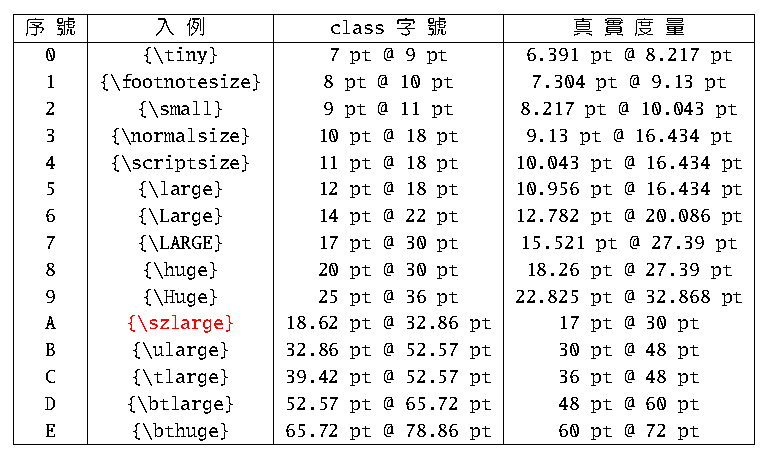
\includegraphics[scale=1]{figures/sz.pdf}}
\end{center}
\par 正文 9 pt 系列,字號不嚴格對應標準字號。
\end{figure}

\begin{figure}[H]
\begin{center}
\caption{正文 9 pt 系列(sz9.cls)}
{ 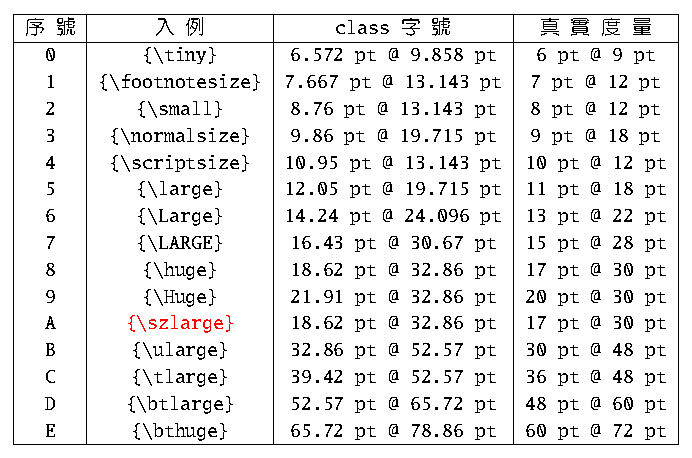
\includegraphics[scale=1]{figures/sz9.pdf}}
\end{center}
\par 正文 9 pt 系列,按此實際字號換算class字號。
\end{figure}

\subsection{正文 10 pt 系列}
\begin{figure}[H]
\begin{center}
\caption{正文 10 pt 系列(sz10.cls)}
{ 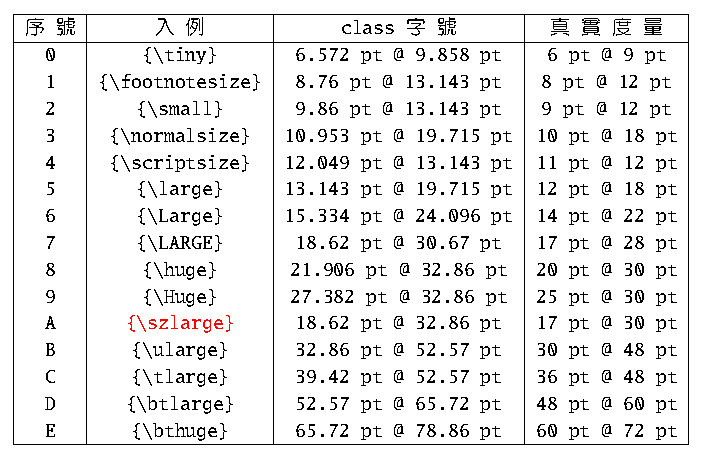
\includegraphics[scale=1]{figures/sz10.pdf}}
\end{center}
\par 正文 10 pt 系列,按此實際字號換算class字號。
\end{figure}

\subsection{正文 11 pt 系列}
\begin{figure}[H]
\begin{center}
\caption{正文 11 pt 系列(sz11.cls)}
{ 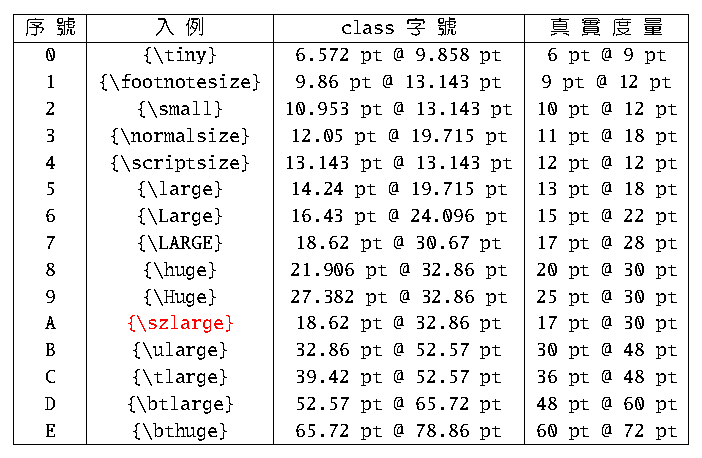
\includegraphics[scale=1]{figures/sz11.pdf}}
\end{center}
\par 正文 11 pt 系列,按此實際字號換算class字號。
\end{figure}


\subsection{正文 12 pt 系列}
\begin{figure}[H]
\begin{center}
\caption{正文 12 pt 系列(sz12.cls)}
{ 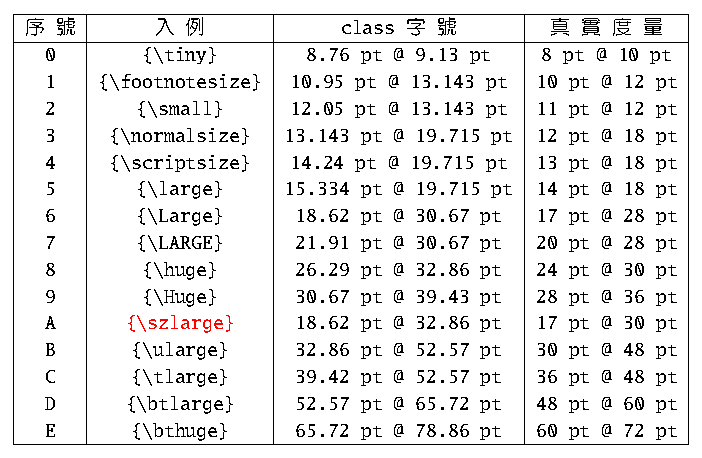
\includegraphics[scale=1]{figures/sz12.pdf}}
\end{center}
\par 正文 12 pt 系列,按此實際字號換算class字號。
\end{figure}

\subsection{正文 五號 系列}
\begin{figure}[H]
\begin{center}
\caption{正文 五號 系列(sz10x.cls)}
{ 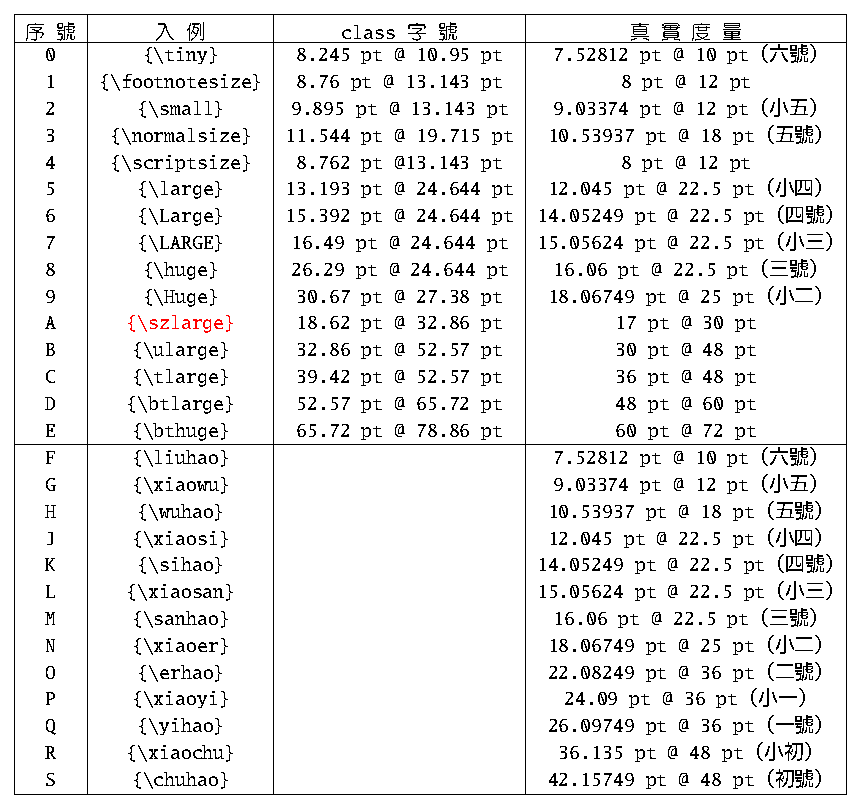
\includegraphics[scale=1]{figures/sz10x.pdf}}
\end{center}
\par 正文  五號  系列,按此實際字號換算class字號。
\end{figure}



\section{up{\LaTeX}常用命令舉例}

\begin{itemize}
\item{}{\verb+\yato+}和{\verb+\tate+}:这两个命令是让你确定横排还是竖排。实际上还有一个{\verb+\dtou+}命令,也是竖排,但是是从下到上,这个命令只有在一些开发文档上才能看到。
\item{}{\verb+\jfont+}和{\verb+\tfont+}:这两个命令和TeX原始的{\verb+\font+}命令一样,但是分别指定的是横排和竖排的字体。在{p\LaTeX}扩展的NFSS编码中,横排和竖排的字体编码为JY1和JT1,{up\LaTeX}中相应的编码为JY2和JT2,{Lua\TeX}-ja中对应的编码为JY3和JT3。
\item{}{\verb+\jfam+}:这个命令是用来定义字体族的,请参考{\TeX}中的{\verb+\fam+}用法。
\item{}{\verb+zh+}和{\verb+zw+}:这两个是相对单位,类似于tfm中定义的ex和em,指的是一个汉字的高度和宽度,定义来源于jfm中的相关部分。
\item{}{\verb+\ybaselineshift+}和{\verb+\tbaselineshift+}:这两个命令是用来对齐汉字和西文之间的基线的,通常情况下都需要进行调整,让汉字与西文对齐。
\item{}{\verb+\kanjiskip+}和{\verb+\xkanjiskip+}:两个命令分别对应的是:汉字-汉字之间距离,汉字-西文距离。 有点像{\TeX}中{\verb+\spaceskip+}(此命令只對西文起作用)。
\item{}{\verb+\kansuji+}和{\verb+\kansujichar+}:前者将阿拉伯数字转换成汉字,如{\verb+\kansuji12+}转换成“一二”。后者给数字指定汉字,如{\verb+\kansujichar1=`壱+}。
\item{}{\verb+\euc+}、{\verb+\jis+}和{\verb+\sjis+}:这个命令相当于{\verb+\char+},就是限定了编码。
\item{}{\verb+\prebreakpenalty+}和{\verb+\postbreakpenalty+}:这两个命令分别在某个字符前或者字符后添加penalty,以达到避头尾的效果。如{\verb+\prebreakpenalty`あ=1000+}。
\item{}{\verb+\jcharwidowpenalty+}:这是控制孤行的。
\item{}{\verb+\xspcode+}:控制{\verb+\xkanjiskip+}插入的命令,对象是西文字符,如{\verb+\xspcode`A=0+}。可选的值为:0,1,2,3。0的情况:禁止在左侧插入。1的情况:允许在左侧插入。2的情况:允许在右侧插入。3的情况:允许两侧插入。
\item{}{\verb+\inhibitglue+}:禁止glue插入。
\item{}{\verb+\autospacing+}和{\verb+\noautospacing+}:允许/禁止汉字-汉字之间插入glue。
\item{}{\verb+\autoxspacing+}和{\verb+\noautoxspacing+}:允许/禁止汉字-西文之间插入glue。
\item{}{\verb+\inhibitxspcode+}:和{\verb+\xspcode+}类似,但是这个命令对象是汉字字符。
\item{}{\verb+\kcatcode+}:类似于TeX的{\verb+\catcode+}。
\end{itemize}

\par\href{https://www.zhihu.com/question/20544732/answer/15437234}%
{詳見``如何使用 LaTeX 輸出豎版排版的文章或書籍?"}


%\clearpage

\section{為up{\LaTeX}配置本地字體}

\subsection{字體實現的三種思路。}
\par\noindent
思路一:通過NFSS設置方法,將已有的tfm及同名vf映射到本地字體。\\
優點:簡單方便,不產生新的vf和tfm,僅適用於臨時占用。\\
缺點:會占用系統預設的tfm和vf。\\[5mm]
思路二:使用PXcopyfont工具包為本地字體複製配套的tfm和vf。\\
優點:為每一個本地字體都配置單獨的vf及tfm,可以避免同系統自帶的tfm及vf撞車;\\
\hspace{3zw}便於移植到下一台計算機。\\
缺點:占用硬盤資源大。配置難度大。\\[5mm]
思路三:使用Jfmutil工具包為本地字體創建全新的tfm和vf。\\
優點:可以自定義禁則。便於移植到下一台計算機。\\
缺點:配置難度太大,禁則編寫難度太高,往往不容易成功。


\subsection{簡體中文字體宏包}
\par
使用\verb+ctex+宏包可以调用Windows/OS X/Linux 本地字体。
使用此package前請先閲讀ctex.pdf 手冊,目前中文繁體支持仍然很差,
除楷體和宋體外,隸書僅支持簡體中文使用。
\begin{lstlisting}[firstnumber=1]
\usepackage[fontset=windows]{ctex}
%\usepackage[fontset=adobe]{ctex}
\end{lstlisting}


\subsection{{up\LaTeXe}字體設置方法(NFSS)}

\par{}使用 八登崇之 PXcopyfont 工具包。(見附件 PXcopyfont 文件夾。)
\par{}安裝 perl 工具包。Windows 10 系統可以下載使用 {ActivePerl}。

\subsubsection*{案例一創建 {kleePro} 虛擬字體和TFM文件}

(請勿照抄此案例。)

\par{}{\bfseries{Windows系統}}在記事本中寫入以下語句,另存為 \uwave{\red{MK KLEE.BAT}}。
\begin{lstlisting}[firstnumber=1]
perl pxcopyfont.pl -o upjisr-h klee-m-jy2 r-klee-m-jy2 r-klee-m-jy2x
perl pxcopyfont.pl -o upjisr-v klee-m-jt2 r-klee-m-jt2
perl pxcopyfont.pl -o jis klee-m-jy1 r-klee-m-jy1
perl pxcopyfont.pl -o jis-v klee-m-jt1 r-klee-m-jt1
perl pxcopyfont.pl -o upjisr-h klee-db-jy2 r-klee-db-jy2 r-klee-db-jy2x
perl pxcopyfont.pl -o upjisr-v klee-db-jt2 r-klee-db-jt2
perl pxcopyfont.pl -o jis klee-db-jy1 r-klee-db-jy1
perl pxcopyfont.pl -o jis-v klee-db-jt1 r-klee-db-jt1
\end{lstlisting}

\par{}保存後,直接雙擊執行。不能用管理員權限,否則進入system32系統文件夾下了。
\par{}現在打開
{\color{red}C:$\backslash$texlive$\backslash$texmf-local$\backslash$fonts$\backslash$vf},
新建klee文件夾,將vf字體複製進去。
\par{}打開
{\color{red}C:$\backslash$texlive$\backslash$texmf-local$\backslash$fonts$\backslash$tfm},
新建klee文件夾,將tfm文件複製進去。
\par{}執行\red{mktexlsr}刷新{\TeX}文件樹。


\subsubsection*{案例二創建 {kleePro} 配置文件}

(請勿照抄此案例。)

\par{}參考{doratex}的博客,在{mysample.tex}中寫入以下語句,使用
{\color{red}\verb+{ptex2pdf -l -u  mysample}+}
進行編譯:
\begin{lstlisting}[firstnumber=1]
%#!使用uplatex 編譯
\documentclass[uplatex]{jsarticle}
\usepackage{plext}% 縦組用
\pagestyle{empty}
%%% klee ファミリーに m と db のシリーズを定義
\DeclareFontFamily{JY2}{klee}{}
\DeclareFontFamily{JT2}{klee}{}

\DeclareFontShape{JY2}{klee}{m}{n}{<->s*[0.924690]klee-m-jy2}{}
\DeclareFontShape{JY2}{klee}{m}{it}{<->ssub*klee/m/n}{}
\DeclareFontShape{JY2}{klee}{m}{sl}{<->ssub*klee/m/n}{}
\DeclareFontShape{JY2}{klee}{m}{sc}{<->ssub*klee/m/n}{}
\DeclareFontShape{JT2}{klee}{m}{n}{<->s*[0.924690]klee-m-jt2}{}
\DeclareFontShape{JT2}{klee}{m}{it}{<->ssub*klee/m/n}{}
\DeclareFontShape{JT2}{klee}{m}{sl}{<->ssub*klee/m/n}{}
\DeclareFontShape{JT2}{klee}{m}{sc}{<->ssub*klee/m/n}{}

\DeclareFontShape{JY2}{klee}{db}{n}{<->s*[0.924690]klee-db-jy2}{}
\DeclareFontShape{JY2}{klee}{db}{it}{<->ssub*klee/db/n}{}
\DeclareFontShape{JY2}{klee}{db}{sl}{<->ssub*klee/db/n}{}
\DeclareFontShape{JY2}{klee}{db}{sc}{<->ssub*klee/db/n}{}
\DeclareFontShape{JT2}{klee}{db}{n}{<->s*[0.924690]klee-db-jt2}{}
\DeclareFontShape{JT2}{klee}{db}{it}{<->ssub*klee/db/n}{}
\DeclareFontShape{JT2}{klee}{db}{sl}{<->ssub*klee/db/n}{}
\DeclareFontShape{JT2}{klee}{db}{sc}{<->ssub*klee/db/n}{}

\DeclareRobustCommand\kleem{\kanjifamily{klee}\kanjiseries{m}\selectfont}
\DeclareRobustCommand\kleedb{\kanjifamily{klee}\kanjiseries{db}\selectfont}

% dvipdfmx special の発行
\AtBeginDvi{%
  \special{pdf:mapline klee-m-jy2    UniJIS2004-UTF16-H FOT-KleePro-M.otf}%
  \special{pdf:mapline klee-m-jt2    UniJIS2004-UTF16-V FOT-KleePro-M.otf}%
  \special{pdf:mapline klee-db-jy2   UniJIS2004-UTF16-H FOT-KleePro-DB.otf}%
  \special{pdf:mapline klee-db-jt2   UniJIS2004-UTF16-V FOT-KleePro-DB.otf}%
}

\begin{document}
\parbox<y>{22zw}{%
{\kleem{}(*クレーミディアムの横組サンプル、「約物の“テスト”」。*)}\par
{\kleedb{}(*クレーデミボールドの横組サンプル、「約物の“テスト”」。*)}}
\vspace{5mm}
\parbox<t>{12zw}{%
{\kleem{}(*クレーミディアムの縦組サンプル、「約物の〝テスト?」。*)}\par
{\kleedb{}(*クレーデミボールドの縦組サンプル、「約物の〝テスト?」。*)}}
\end{document}
\end{lstlisting}

\begin{figure}[H]
\par\quad\marg{出力例:}
\begin{center}
\fbox{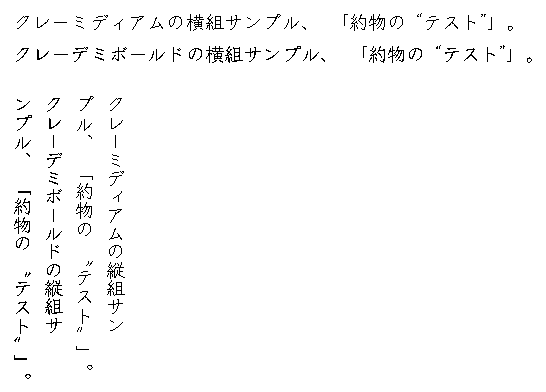
\includegraphics[width=0.6\textwidth]{figures/06.pdf}}
\end{center}
\end{figure}

%\clearpage
\subsection{簡體中文本地字體}

\par{}參照前文
配置虛擬字體和tfm。然後指定mapline為{UniGB-UTF16-H}和{UniGB-UTF16-V},
或者{UniGB-UCS2-H}和{UniGB-UCS2-V}。 或者使用 {unicode}作爲{mapline}。
示例如下:

\begin{lstlisting}[firstnumber=1]
  \special{pdf:mapline fzks-m-jy2   unicode  FZKSGBXS10.ttf}% 方正楷書 (*GB18030-S10*)版
  \special{pdf:mapline fzks-m-jt2   unicode  FZKSGBXS10.ttf -w 1}% -w 1 表示垂直排版模式
  \special{pdf:mapline fzks-sip-m-jy2   unicode  FZKaiS(SIP).TTF}%方正楷書(*S-SIP(CJK-B版)*)
  \special{pdf:mapline fzks-sip-m-jt2   unicode  FZKaiS(SIP).TTF -w 1}%
  \special{pdf:mapline fzxss-m-jy2   UniGB-UTF16-H  FZXSSGBX.TTF}% 方正新書宋 GB18030
  \special{pdf:mapline fzxss-m-jt2   UniGB-UTF16-V  FZXSSGBX.TTF}%
\end{lstlisting}

\subsection{使用{Pxchfon}宏包配置日文版思源字體}
\par{}在{mysample.tex}中寫入以下語句:

\begin{lstlisting}[firstnumber=1]
\usepackage[uplatex,deluxe]{otf}               % 多字重支持
%\usepackage[sourcehan]{pxchfon}                 % 不使用 JIS2004 字形
\usepackage[sourcehan,prefer2004jis]{pxchfon}    %   使用 JIS2004 字形

\setminchofont{SourceHanSerif-Medium.otf}
\setlightminchofont{SourceHanSerif-Regular.otf}
\setboldminchofont{SourceHanSerif-Bold.otf}
\setgothicfont{SourceHanSans-Medium.otf}
\setmediumgothicfont{SourceHanSans-Regular.otf}
\setboldgothicfont{SourceHanSans-Bold.otf}
\setxboldgothicfont{SourceHanSans-Heavy.otf}
\setmarugothicfont{SourceHanSans-Regular.otf}
\end{lstlisting}

(行5 - 12 是 sourcehan 選項時預設的,與之等價,詳見 pxchfon.pdf)

\begin{table}[H]
\begin{center}
\caption{pxchfon 宏包等價命令}
{\fontsize{8pt}{12}\selectfont\ttfamily
\begin{tabular}{|l|l|l|}
 \hline
 \multicolumn{1}{|c|}{OTF/TTF 命令} & \multicolumn{1}{|c|}{TTC 命令} & \multicolumn{1}{|c|}{用途} \\ \hline
$\backslash$setminchofont\{*.otf/*.ttf\} & $\backslash$setminchofont[番號]\{*.ttc\} & 設置正文明朝體;\\
$\backslash$setlightminchofont\{*.otf/*.ttf\} & $\backslash$setlightminchofont[番號]\{*.ttc\} & 設置細明朝體;\\
$\backslash$setboldminchofont\{*.otf/*.ttf\} & $\backslash$setboldminchofont[番號]\{*.ttc\} & 設置粗明朝體;\\
$\backslash$setgothicfont\{*.otf/*.ttf\} & $\backslash$setgothicfont[番號]\{*.ttc\} & 設置哥特體(細黑體);\\
$\backslash$setmediumgothicfont\{*.otf/*.ttf\} & $\backslash$setmediumgothicfont[番號]\{*.ttc\} & 設置中等哥特體;\\
$\backslash$setboldgothicfont\{*.otf/*.ttf\} & $\backslash$setboldgothicfont[番號]\{*.ttc\} & 設置粗哥特體;\\
$\backslash$setxboldgothicfont\{*.otf/*.ttf\} & $\backslash$setxboldgothicfont[番號]\{*.ttc\} & 設置特粗哥特體;\\
$\backslash$setmarugothicfont\{*.otf/*.ttf\} & $\backslash$setmarugothicfont[番號]\{*.ttc\} & 設置丸書體(即圓體)。\\ \hline
\end{tabular} }
\end{center}
\end{table}


\subsection{東亞字體CMAP簡介}
\par{}CMAP是對字符映射起到索引作用的文件。(見表3)

\subsection{CID-Key和CID符號}

\par{}{up\LaTeXe}自帶一些系統命令,可以調用系統字體(如小塚明朝 kozuka-pr6n)的CID字和符號。
具體CID編號需檢索技術文檔{5078.Adobe-Japan1-6.pdf},網頁搜索即可獲取。相關示例(見表4)


\begin{table}[H]
\caption{東亞字體CMAP簡介}
{\fontsize{8pt}{12}\selectfont\ttfamily
\begin{tabular}{|c|l|l|c|l|}
\hline
 \multicolumn{1}{|c|}{言 語} & \multicolumn{1}{|c|}{CMAP(橫)}%
  &\multicolumn{1}{|c|}{CMAP(縱)}& \multicolumn{1}{|c|}{工具引擎} & \multicolumn{1}{|c|}{備注} \\ \hline
日本語& 2004-H & 2004-V & {p\LaTeX}、{p\TeX} & 適用於JIS2004字形 \\
日本語& UniJIS-UTF16-H & UniJIS-UTF16-V & {up\LaTeX}、{Up\TeX} & 適用於JIS90字形 \\
日本語& UniJIS2004-UTF16-H & UniJIS2004-UTF16-V & 同上 & 適用於JIS2004字形 \\
日本語& UniSourceHanSansJP-UTF16-H & UniSourceHanSansJP-UTF16-V & 同上 & 源ノ角ゴシック (思源黑體日版) \\
日本語& UniSourceHanSerifJP-UTF16-H & UniSourceHanSerifJP-UTF16-V & 同上 & 源ノ明朝(思源明體日版) \\ \hline
簡體中文& UniSourceHanSansCN-UTF16-H & UniSourceHanSansCN-UTF16-V & 同上 & 思源黑體 \\
簡體中文& UniSourceHanSerifCN-UTF16-H & (無,用unicode替代) & 同上 & 思源宋體 \\
簡體中文& UniGB-UTF16-H & UniGB-UTF16-V & 同上 & 適用於簡體 \\
簡體中文& UniGB-UCS2-H & UniGB-UCS2-V & 同上 &  \\ \hline
繁體中文& UniSourceHanSansTW-UTF16-H & (無,用unicode替代) & 同上 & 思源黑體台版 \\
繁體中文& UniSourceHanSerifTW-UTF16-H & (無,用unicode替代) & 同上 & 思源宋體台版 \\
繁體中文& UniCNS-UTF16-H & UniCNS-UTF16-V & 同上 & 適用於繁體 \\
繁體中文& UniCNS-UCS2-H & UniCNS-UCS2-V & 同上 &  \\ \hline
韓國語& (無,用unicode替代) & (無,用unicode替代) & 同上 & 思源黑體韓版 \\
韓國語& 同上 & 同上 & 同上 & 思源明體韓版 \\
韓國語& UniKS-UTF16-H & UniKS-UTF16-V & 同上 &  \\ \hline
\end{tabular} }
\end{table}



\begin{table}[H]
\begin{center}
\caption{Adobe-Japan1-6 使用CID鍵調用特殊符號 示例}
\begin{tabular}{|c|c|c|}
\hline
 入例 & 出例 & 說明\\ \hline
\verb+\CID{1260}+ & \CID{1260} & “永”字 \\
\verb+\CID{119}+ & \hskip.3zw\CID{119} & 垂直磅點,用於縱書 \\
\verb+\CID{8015}+ & \CID{8015} & 圓角方框 \\
\verb+\CID{779}+ & \CID{779} & 圓圈號 \\
\verb+\CID{731}+ & \CID{731} & 上三角 \\
\verb+\CID{733}+ & \CID{733} & 下三角 \\ \hline
\end{tabular}
\end{center}
\end{table}



\section{注意事項}

\par%
使用pxchfon包調用思源日版OTF字體時,默認采用jis2004的標點符號,即將逗號%
(,)轉寫為讀點(、)。而縱排時,jis2004的頓號是用的磅點(\verb+\CID{119}+),
此符號在橫排中只占據半角字寬。

\vspace{5mm}
\par%
使用 {\color{red}\verb+ptex2pdf -l -u -ot "-kanji=utf8 "  -od "-p B5" mysample+}
 命令編譯 PDF ,則會調用 ISO B5 紙張。實際紙張為 JIS B5。印前檢査時若不允許放縮,
 則應思考縮小版心尺寸,並縮小頁面尺寸及頁邊距。再次印前檢査時,使用{\color{red}\verb+100 % +} 放縮比例,
 製作裁切及出血標記。

\subsection{已知問題}

\begin{enumerate}
\item 使用{\color{red}\verb+\setlength{\parindent}{2zw}+}或者
{\color{red}\verb+\setlength{\parindent}{2em}+} 不會改變段落縮進。
默認段落縮進為一個全角漢字。\\
解決辦法:在\verb+\begin{document}+後面使用{\color{red}\verb+\setlength{\parindent}{2zw}+}。
\item 部標題既不是水平居中,也不是垂直居中。
\end{enumerate}

\subsection{常見錯誤}
\begin{enumerate}
\item {\mc\bfseries{}問題一:找不到TFM,或者vf。}\\
解決辦法:査找你的tfm、vf、以及字體配置文件。tfm和vf必須一一對應,
而且配置文件裏頭不能寫錯了。比如大小寫錯,以及寫反、漏寫之類。

\item {\mc\bfseries{}問題二:出現豆腐塊。字體無法正確顯示。}\\
解決辦法:試圖尋找能顯示這個字的字體,并且爲之配置簡體中文。

\item {\mc\bfseries{}問題三:看不到pdf,控制台一閃而過。}\\
解決辦法:在脚本中加入一行 pause。使之在退出之前保持錯誤信息。

\item {\mc\bfseries{}問題四:}\\
\verb+{\contentsline {section}{\numberline {5}...+\\
\verb+! File ended while scanning use of \@writefile.+\\
\verb+<inserted text>+\\



解決辦法:先排査錯誤,刪除臨時文件,再重新編譯。
\item {\mc\bfseries{}問題五:Windows 10 CMD 控制台 顯示漢字亂碼。}\\
解決辦法:打開 {\color{red}編譯.bat},在第一行寫入 {\color{red}chcp 65001}。
\hspace{.5zw}65001 表示將控制台編碼切換到Unicode。

\item {\mc\bfseries{}問題六:自定義的字體無法準確切換到下一行,行尾參差不齊。}\\
解決辦法:打開PXcopyfont$>$TFM-source,將upstsl-h.tfm和upstsl-v.tfm 重命名為
自定義字體的tfm名稱,替換掉出錯的tfm文件。注意h/v 一定要對應。
一般采納JY2/JT2為{up\LaTeX}橫排和縱排時使用的字體。
我們將upstsl-h.tfm改成foobar-jy2.tfm,upstsl-v.tfm改成foobar-jt2.tfm,
替換掉出錯的tfm文件。

\end{enumerate}

\section{致謝}
\par%
感謝熊本学園大学経済学部{小川\hskip1zw 弘和}老師。
\par%
感謝湘南情報数理化学研究所{藤田\hskip1zw 眞作}老師。
\par%
感謝{阿部\hskip1zw 紀行}老師。
\par%
感謝{八登\hskip1zw 崇之}老師。
\par%
感謝大阪大學{金水\hskip1zw 敏}老師。

%\clearpage

\section{參考鏈接}

\par\href{http://www2.kumagaku.ac.jp/teacher/herogw/}{JIS X0212 for pTeX - 熊本学園大学}
%\vspace{5mm}
\par%
\href{http://abenori.blogspot.com/2016/07/warichu-eplatex.html}{阿部紀行氏 jlreq.class 提取,warichus.sty 實裝 。}

%\vspace{5mm}
\par\href{http://xymtex.com/fujitas2/texlatex/index.html}{藤田眞作氏 頭注 下載網頁。}

%\vspace{5mm}

\par%

\href{https://texwiki.texjp.org/?LaTeX%20%E3%81%AE%E3%82%A8%E3%83%A9%E3%83%BC%E3%83%A1%E3%83%83%E3%82%BB%E3%83%BC%E3%82%B8}{{up\LaTeX} 常見錯誤集錦。\LaTeX のエラーメッセージ。}

\par%
{up\LaTeX} 字體配置相關參考網頁:
\par\url{https://qiita.com/zr_tex8r/items/15ec2848371ec19d45ed}
\par\url{https://qiita.com/zr_tex8r/items/5c14042078b20edbfb07}
\par\url{http://doratex.hatenablog.jp/entry/20161206/1480950097}

\endinput


\clearpage

\section*{附\quad 錄}

\begin{appendix}

\section{up\LaTeX 字體的配置}
\par  通常,up\LaTeX 使用{\bfseries dvipdfmx package } 進行pdf 輸出 ,
您可以先嘗試使用以下命令瀏覽本機支持的東亞漢字字族。\\
※ 請\hspace{3pt}以\red{管理員權限執行} ,
OS X / Linux系統中使用 \red{\bfseries sudo} 十分必要。
\begin{lstlisting}[firstnumber=1]
kanji-config-updmap-sys status
\end{lstlisting}

系統會回顯您的電腦上可用的字族。如下:
\begin{lstlisting}[firstnumber=1]
C:\Windows\system32>kanji-config-updmap-sys status
CURRENT family for ja: kozuka-pr6n
Standby family : ipa
Standby family : ipaex
Standby family : kozuka
Standby family : ms
Standby family : yu-win10
\end{lstlisting}

然後使用以下命令設置:
\begin{lstlisting}[firstnumber=1]
(* \CID{234} ※ Unix的OSの場合, sudoが必要 *)

(* \CID{234} IPAexフォントを使う *)
$ kanji-config-updmap-sys ipaex

(* \CID{234} macOS(El Capitan以降)付属のヒラギノフォントを使う *)
$ kanji-config-updmap-sys hiragino-elcapitan-pron

(* \CID{234} 小塚フォント(Pr6N版)を使う; 舊字形 *)
$ kanji-config-updmap-sys  kozuka-pr6n
(*或*)
(* \CID{234} 小塚フォント(Pr6N版)を使う; 2004JIS字形指定 *)
$ kanji-config-updmap-sys --jis2004 kozuka-pr6n
\end{lstlisting}
\par 推薦使用{\bfseries  kanji-config-updmap-sys --jis2004 kozuka-pr6n}.
\par {\bfseries  --jis2004} 選項:是否使用JIS2004標準字形。無此選項則表示
采用{\bfseries{}JIS90}字形。相關信息詳細請檢索網頁,此處不再贅述。
\par 關於字族的説明:
\begin{table}[H]
\begin{center}
\begin{tabular}{p{30mm}p{120mm}}
\hline
\CID{119} kozuka-pr6n  & 小塚フォント(小塚明朝 Pr6N版),非商用 \\
\CID{119} ipa  & 独立行政法人情報処理推進機構開發的 IPA 舊字 \\
\CID{119} ipaex  &  独立行政法人情報処理推進機構
開發的 IPA 新字體\footnotemark[3] \\
\CID{119} kozuka  &  小塚フォント(小塚明朝),非商用\\
\CID{119} ms   &  Microsoft系統附贈,非商用\\
\CID{119} yu-win10   &   Microsoft日文版Windows系統附贈字體,
需從網頁下載使用,非商用 \\ \hline
\end{tabular}
\end{center}
\end{table}

\footnotetext[3]{IPAex字體下載地址:\url{https://ipafont.ipa.go.jp/node26} }



\par 設置結果如下所示:
\begin{lstlisting}[firstnumber=1]
C:\Windows\system32>kanji-config-updmap-sys kozuka-pr6n
Setting up ... ptex-kozuka-pr6n.map
... ...
Generating output for dvipdfmx...
Generating output for ps2pk...
Generating output for dvips...
Generating output for pdftex...
... ...
c:/texlive/2018/texmf-var/fonts/map/dvipdfmx/updmap:
7726 2019-01-09 01:39:07 kanjix.map
Transcript written on "c:/texlive/2018/texmf-var/web2c/updmap.log".
updmap: Updating ls-R files.
C:\Windows\system32>
\end{lstlisting}
\par 這樣就表示您的字體設置成功了。

%\clearpage

\section{ptex2pdf使用參數紹介}\label{ptex2pdf}

\begin{lstlisting}[firstnumber=1]
[texlua] ptex2pdf[.lua] { option | basename[.tex] } ...
\end{lstlisting}
{ \bfseries  options:}
\begin{table}[H]
\begin{center}
\begin{tabular}{p{90mm}p{60mm}}
\hline
\CID{119}  -v  version  & 顯示版本\\
\CID{119}  -h  help  & 幫助\\
\CID{119}  -help print full help (installation, TeXworks setup) & \\
\CID{119}  -e  use eptex class of programs  & 使用ep\TeX 特性進行編譯\\
\CID{119}  -u  use uptex class of programs & 使用up\TeX 特性進行編譯\\
\CID{119}  -l  use latex based formats  & 引用\LaTeX 語法格式\\
\CID{119}  -s  stop at dvi  & 編譯結束,在dvi之前立即停止\\
\CID{119}  -i  retain intermediate files  & 保留過程文件\\
\CID{119}  -ot $<opts>$ extra options for  \TeX   & 額外 \TeX 選項\\
\CID{119}  -od $<opts>$ extra options for dvipdfmx  & 額外 dvipdfmx 選項\\
\CID{119}  -output-directory $<dir>$ directory for created files  & 指定pdf 輸出 目錄\\ \hline
\end{tabular}
\end{center}
\end{table}

\section{up{\LaTeX}常用命令舉例}
\symkm
\begin{itemize}
\item{}{\verb+\yato+}和{\verb+\tate+}:这两个命令是让你确定横排还是竖排。实际上还有一个{\verb+\dtou+}命令,也是竖排,但是是从下到上,这个命令只有在一些开发文档上才能看到。
\item{}{\verb+\jfont+}和{\verb+\tfont+}:这两个命令和TeX原始的{\verb+\font+}命令一样,但是分别指定的是横排和竖排的字体。在{p\LaTeX}扩展的NFSS编码中,横排和竖排的字体编码为JY1和JT1,{up\LaTeX}中相应的编码为JY2和JT2,{Lua\TeX}-ja中对应的编码为JY3和JT3。
\item{}{\verb+\jfam+}:这个命令是用来定义字体族的,请参考{\TeX}中的{\verb+\fam+}用法。
\item{}{\verb+zh+}和{\verb+zw+}:这两个是相对单位,类似于tfm中定义的ex和em,指的是一个汉字的高度和宽度,定义来源于jfm中的相关部分。
\item{}{\verb+\ybaselineshift+}和{\verb+\tbaselineshift+}:这两个命令是用来对齐汉字和西文之间的基线的,通常情况下都需要进行调整,让汉字与西文对齐。
\item{}{\verb+\kanjiskip+}和{\verb+\xkanjiskip+}:两个命令分别对应的是:汉字-汉字之间距离,汉字-西文距离。 有点像{\TeX}中{\verb+\spaceskip+}(此命令只對西文起作用)。
\item{}{\verb+\kansuji+}和{\verb+\kansujichar+}:前者将阿拉伯数字转换成汉字,如{\verb+\kansuji12+}转换成“一二”。后者给数字指定汉字,如{\verb+\kansujichar1=`壱+}。
\item{}{\verb+\euc+}、{\verb+\jis+}和{\verb+\sjis+}:这个命令相当于{\verb+\char+},就是限定了编码。
\item{}{\verb+\prebreakpenalty+}和{\verb+\postbreakpenalty+}:这两个命令分别在某个字符前或者字符后添加penalty,以达到避头尾的效果。如{\verb+\prebreakpenalty`あ=1000+}。
\item{}{\verb+\jcharwidowpenalty+}:这是控制孤行的。
\item{}{\verb+\xspcode+}:控制{\verb+\xkanjiskip+}插入的命令,对象是西文字符,如{\verb+\xspcode`A=0+}。可选的值为:0,1,2,3。0的情况:禁止在左侧插入。1的情况:允许在左侧插入。2的情况:允许在右侧插入。3的情况:允许两侧插入。
\item{}{\verb+\inhibitglue+}:禁止glue插入。
\item{}{\verb+\autospacing+}和{\verb+\noautospacing+}:允许/禁止汉字-汉字之间插入glue。
\item{}{\verb+\autoxspacing+}和{\verb+\noautoxspacing+}:允许/禁止汉字-西文之间插入glue。
\item{}{\verb+\inhibitxspcode+}:和{\verb+\xspcode+}类似,但是这个命令对象是汉字字符。
\item{}{\verb+\kcatcode+}:类似于TeX的{\verb+\catcode+}。
\end{itemize}

\mcfamily

\par\href{https://www.zhihu.com/question/20544732/answer/15437234}%
{詳見``如何使用 LaTeX 輸出豎版排版的文章或書籍?"}

\section{ Drag&Drop Up\TeX 2018介紹}\label{uptex-xiongben}

配置緊湊(具體來說,TeX Live 方案 - 小到只收集日語解決方案),
但它足以使用 p\LaTeX 和 up\LaTeX。 此外,它還帶有一個自動執行
日語字體設置的 GUI,因此您可以用最少的操作完成日語字體設置。
通過將 \TeX 環境包裝在應用程序包中,使用拖放功能將其安裝在
任意位置,並以最少的操作完成必要的設置。

\CID{722}OSX 專用。

項目網站:\url{http://www2.kumagaku.ac.jp/teacher/herogw/}

\clearpage
\section{中日文字分級簡介}
\subsection{日本文字分級}
{\gtfamily
代表字體: Kozuka-Mincho-Pr6;Kozuka-Gothic-Pr6;\\
\qquad \qquad \qquad Kozuka-Mincho-Pr6N;Kozuka-Gothic-Pr6N;}

\begin{table}[h]
\caption{\fontsize{12pt}{15pt}\selectfont Adobe-Japan1 編碼覆蓋範圍} % title of Table
\centering % used for centering table
\begin{tabular}{|c|c|p{8cm}|c|}% 通过添加 | 来表示是否需要绘制竖线
\hline  % 在表格最上方绘制横线

規格 & 慣用的な商品記号	& \multicolumn{1}{|c|}{おおよその特徴 / 該当製品の例} & 文字数(漢字数) \\

\hline  %在第一行和第二行之间绘制横线
AJ1-0 &	─	 & 漢字 Talk (昔の Mac OS)
をベースに、新旧 (1978 ? 1983) の JIS 第 1 水準?第 2 水準漢字をカバー。
& 8,284 (6,653) \\
\hline
AJ1-1	& ─ &	当時制定された JIS90 に対応。
AJ1-0 と大差なし。 & 	8,359 (6,655) \\
\hline
AJ1-2	& ─	 &  IBM 選定文字 (Win 機種依存文字)
に対応。これにより当時の Win ? Mac で一般的だった文字を共にカバー。
& 	8,720 (7,014) \\
\hline

AJ1-3	& Std/StdN	&   AJ1-2 に記号などを追加。
漢字の追加はなし。ヒラギノフォント?イワタ書体ライブラリー?ダイナフォ
ント?モトヤ?モリサワ?タイプバンク (旧リョービ製品含む) ?カタオカデザ
インワークス? Font-Kai ?清和堂 & 9,354 (7,014) \\

\hline
AJ1-4	& Pro/ProN &
(ヒラギノを除く)	商業印刷で必要になる主だった漢字
(人名?学術漢字など) や大量の記号を追加。
モトヤ?イワタ書体ライブラリー?モリサワ?タイプバンク
(旧リョービ製品含む)  & 15,444 (9,138) \\
\hline
AJ1-5	& Pr5/Pr5N &
(ヒラギノは Pro/ProN、
ダイナフォントは Pro-5)	使用頻度の低い漢字を大量追加。
これにより、JIS 第 3 ?第 4 水準漢字をカバー。
ヒラギノフォント?ビープラス?モリサワ?タイプバンク
(旧リョービ製品含む) ?ダイナフォント  & 20,317 (12,676) \\

\hline
AJ1-6	& Pr6/Pr6N	&  JIS 補助漢字 (1990)
の残りなど、更に使用頻度の低い漢字を追加。これにより JIS 拡張漢字
(2004) をカバー。ヒラギノフォント?イワタ書体ライブラリー?モリサワ
& 23,058 (14,663) \\

\hline
AJ1-7	& Pr7/Pr7N	&  因改元需增加一橫一縱兩個年號合字。 & 增改未詳 \\

\hline % 在表格最下方绘制横线
\end{tabular}

\end{table}

\clearpage
\subsection{簡體中文分級}
{\gtfamily 代表字體: AdobeKaitiStd-Regular.otf ;AdobeSongStd-Light.otf;\\
\qquad \qquad \qquad AdobeHeitiStd-Regular.otf;AdobeFangsongStd-Regular.otf}
\begin{table}[h]
\caption{\fontsize{12pt}{15pt}\selectfont Adobe-GB1 編碼覆蓋範圍} % title of Table
\centering % used for centering table
\begin{tabular}{|c|c|p{8cm}|c|}% 通过添加 | 来表示是否需要绘制竖线
\hline  % 在表格最上方绘制横线

規格 & 商品記号	& \multicolumn{1}{|c|}{特 徴} & 文字数(漢字数) \\

\hline  %在第一行和第二行之间绘制横线
Adobe-GB1-0 &	GB0	 & 1995年6月26日發佈,
共計7717個CID,主要爲GB2312編碼,簡體中文。
& 7,717 (6,762) \\
\hline
Adobe-GB1-1	& GB1 &	1996年2月6日發佈,
計2,180個CID,GB/T12345-90繁體字符集。
& 	9,897 (8,941) \\
\hline
Adobe-GB1-2	& GB2	 &  1997年11月13日發佈,
計12,230個CID,主要支持GBK(GB13000.1-93)編碼,
符合Unicode 2.1規範。 & 22,127 (20,995) \\
\hline

Adobe-GB1-3	& GB3	&   1998年10月8日發佈,
計226個CID,主要是旋轉的拉丁文字,
用於縱向排列。 & 22,353 (20,995) \\

\hline
Adobe-GB1-4	& GB4 & 2000年11月20日發佈,
計6,711 個CID,支持GN18030-2000編碼,
滿足Unicode 3.0標準,ISO10646-1:2000以及 CJK-ext-A區的全部文字。
& 29,064 (27,625) \\
\hline
Adobe-GB1-5	& GB5 & 主要是彜族文字,來自GB18030-2005字符集,
計1,220個CID & 30,284(27,625) \\

\hline % 在表格最下方绘制横线
\end{tabular}

\end{table}


\subsection{繁體中文分級}
{\gtfamily 代表字體:AdobeMingStd-Light.otf ;AdobeFanHeitiStd-Bold.otf;}
\begin{table}[h]
\caption{\fontsize{12pt}{15pt}\selectfont Adobe-CNS1 編碼覆蓋範圍} % title of Table
\centering % used for centering table
\begin{tabular}{|c|c|p{8cm}|c|}% 通过添加 | 来表示是否需要绘制竖线
\hline  % 在表格最上方绘制横线

規格 & 商品記号	& \multicolumn{1}{|c|}{特 徴} & 文字数(漢字数) \\

\hline  %在第一行和第二行之间绘制横线
Adobe-CNS1-0 &	-	 & 1995年6月26日發佈,共計14,099個CID,
主要爲CNS11643-1992規範一面、二面,BIG5編碼,繁體中文。
& 14,099 (13,098) \\
\hline
Adobe-CNS1-1	& - &	1998年9月發佈,計3,309個CID,HK-GCCS擴展集。
& 	17,408 (16,382) \\
\hline
Adobe-CNS1-2	& - &  1998年10月12日發佈,
計193個CID,主要主要是旋轉的拉丁文字,
用於縱向排列。 & 17,601 (16,382) \\
\hline

Adobe-CNS1-3	& -	&   2000年6月發佈,計1,245個CID,
包括歐文和HK-SCS-1999標準的字符。
&  18,846 (17,558) \\

\hline
Adobe-CNS1-4	& CNS4 & 2001年8月發佈,計119個CID,
其中116個為HK-SCS-2001標準。
& 18,965(17,676) \\
\hline
Adobe-CNS1-5	& CNS5 & 2005年7月8日發佈,計123個CID,
來自HK-SCS-2004標準。 & 19,088(17,799) \\
\hline
Adobe-CNS1-6	& CNS6 & 2009年9月24日發佈。
來自HK-SCS-2008標準,計68個CID. & 19,156(17,867) \\
\hline % 在表格最下方绘制横线
\end{tabular}

\end{table}

\end{appendix}

% 輸入封底

\clearpage
\thispagestyle{empty}


	\begin{center}
\begin{minipage}<y>[htpb]{125mm}
\vspace{180mm} %奥付のページ上部からの位置
\fontsize{10pt}{25}\mcfamily
		\begin{tabular}{l}
			\multicolumn{1}{c}{\Large{\mcfamily\bfseries\kanjiskip=2pt{up\LaTeX}{小川弘和}{SZ.CLS}{説明}}}\\[3mm] %%タイトル
				\hline
				%\\[3mm]
			\hspace{2mm}\makebox[5zw][s]{著 者}\hspace{5mm}%
			子\hskip1zw 康(SteveCheung)\\[0mm]  %%著者
			\hspace{2mm}\makebox[5zw][s]{発 行 日}\hspace{5mm}\today\\[0mm] %%発行日。「(西元\number\year~年\number\month~月\number\day~日)」のところに任意の日付を入れてもいい。
			\hspace{2mm}\makebox[5zw][s]{発 行 者}\hspace{5mm}%
			{子\hskip1zw 康(SteveCheung)}\\[0mm]  %%発行者
			\hspace{2mm}\makebox[5zw][s]{聯絡方式}\hspace{5.2mm}%
			{dongfang0571@gmail.com}\hspace{30mm}%
									\normalsize{\upstht{\CID{734}商用允許(保留署名);轉載自由 }}
			 %\\[3mm]  %%発行者
				\\\hline
		\end{tabular}
\end{minipage}
	\end{center}

\endinput




\end{document}

